\chapter{Utilização do sistema}
\label{cha:utilizacao}

Neste capítulo descrevemos inicialmente a utilização do sistema. A descrição tende
a ser sucinta, visto que a ferramenta é bastante simples e as telas são auto-explicativas.
Posteriormente, descrevemos os principais passos para a instalação e configuração
do sistema no servidor web.

\section{Utilização do sistema}
O TCC-Manager consiste de vários módulos, que possuem comportamentos diferentes dependendo do 
tipo de usuário que está autenticado no sistema. São 4 (quatro) perfis possíveis:
\begin{itemize}
\item[Administrador] Adminstrador do sistema. Cabe a este perfil cadastrar alunos e professores.
Ele também tem acesso somente-leitura às propostas e defesas.
\item[Estudante] Possui acesso somente a manutenção de seus próprios projetos.
\item[Professor] Possui acesso às propostas e solicitações de defesa de seus orientandos.
\item[Comissão] Possui acesso a todas as propostas e solicitações de defesa do sistema.
\end{itemize}

Devido a essas diferenças de perfis, dividiremos a utilização do sistema de acordo com cada um.

\subsection{Telas em comum entre todos os perfis}
A tela de acesso ao sistema (Figura ~\ref{fig:tela_login}) e a tela de acesso negado (Figura ~\ref{fig:tela_acesso_negado}) são as mesmas para todos os perfis.
Na tela de acesso ao sistema (Figura ~\ref{fig:tela_login}), o campo login espera receber o nome de usuário
para todos os perfis exceto para estudantes, que devem digitar a sua matrícula.

A tela de acesso negado (Figura ~\ref{fig:tela_acesso_negado}) é exibida quando um usuário tenta acessar uma tela de outro perfil, sem
ter a permissão necessária para isso.

\begin{figure}[htbp]
\centering

\includegraphics[width=1\textwidth]{fig/telas/login.png}
\caption{Tela de acesso ao sistema}
\label{fig:tela_login}
\end{figure}

\begin{figure}[htbp]
\centering
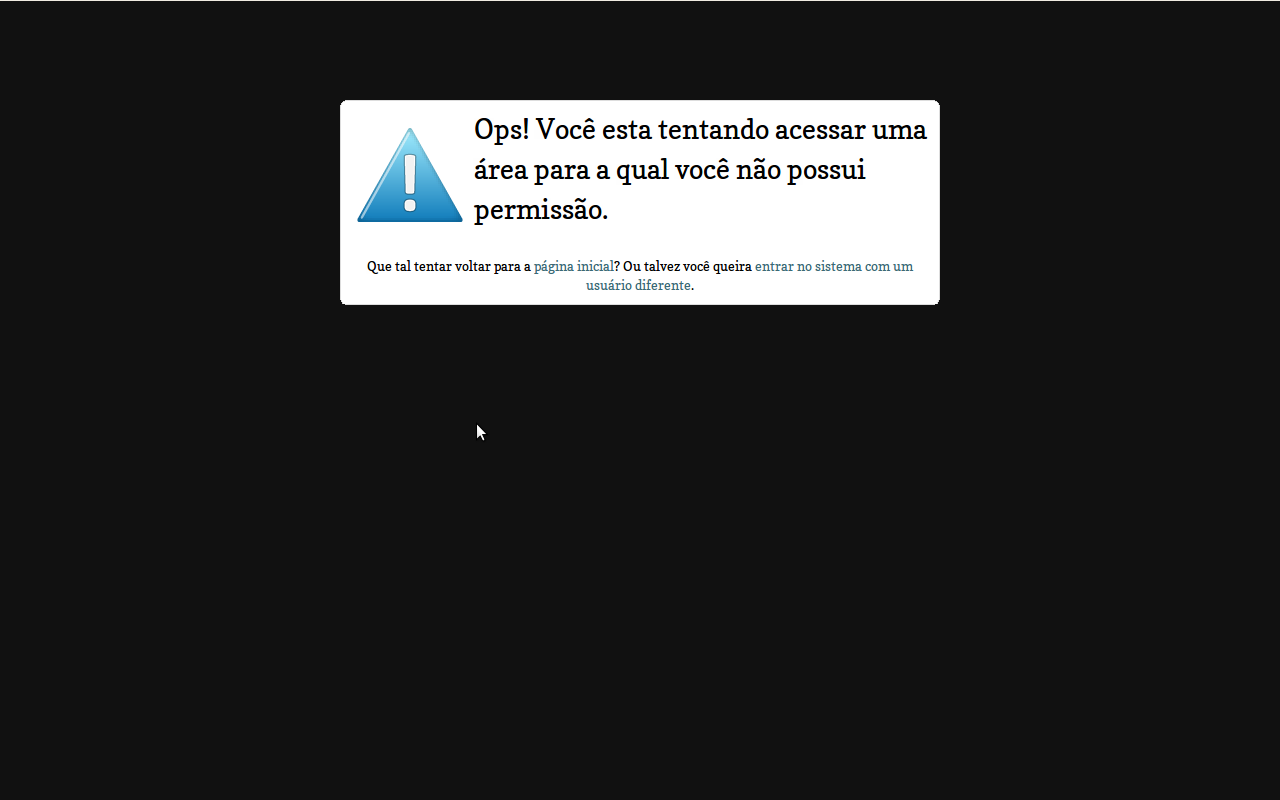
\includegraphics[width=1\textwidth]{fig/telas/acesso_negado.png}
\caption{Tela de acesso negado}
\label{fig:tela_acesso_negado}
\end{figure}


\subsection{Perfil de administrador}
O perfil do administrador consiste basicamente dos cadastros do sistema. A seguir veremos as
telas de cadastro de professores, alunos e semestres. Em seguida vemos que este perfil também
pode visualizar quais propostas e defesas estão cadastradas no banco de dados e pode 
consultar relatórios.

\begin{figure}[htbp]
\centering
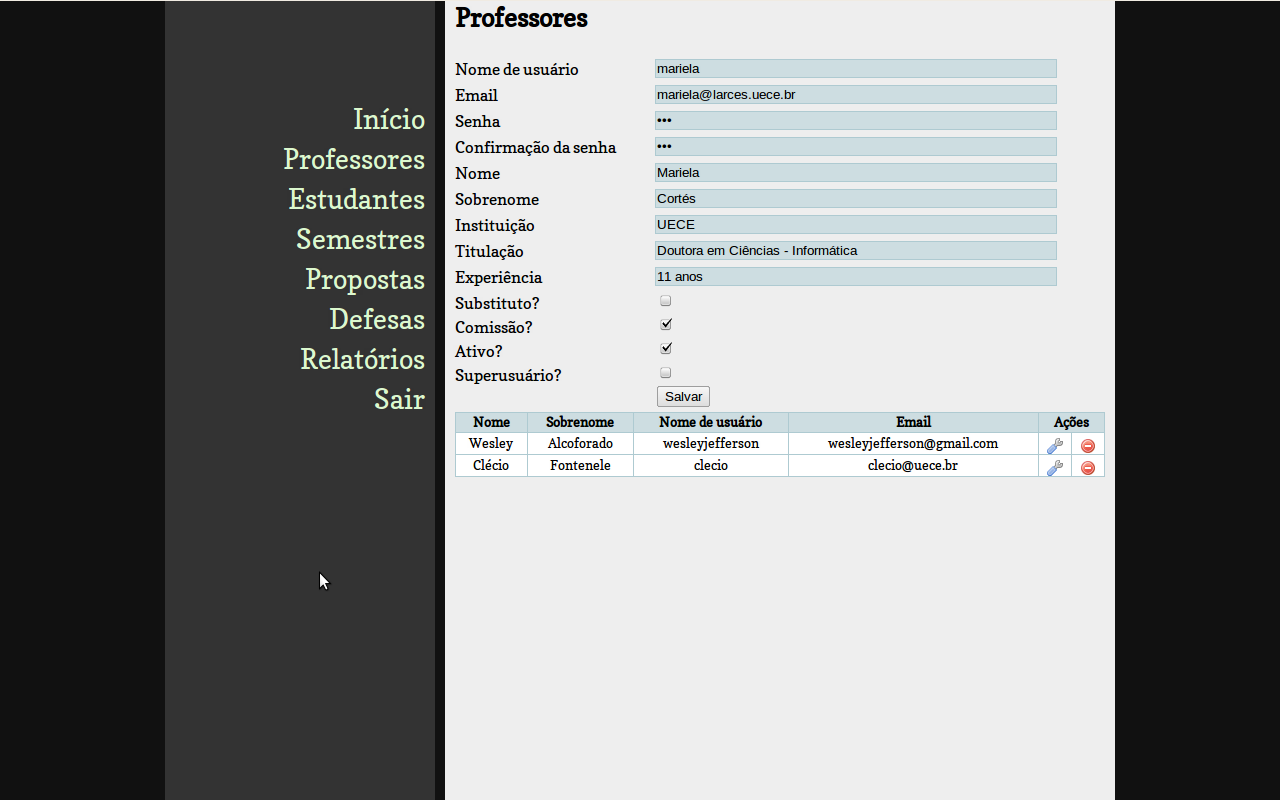
\includegraphics[width=1\textwidth]{fig/telas/administrador/crud_professor_insercao.png}
\caption{Tela de cadastro de professores}
\label{fig:crud_professor_insercao}
\end{figure}

\begin{figure}[htbp]
\centering
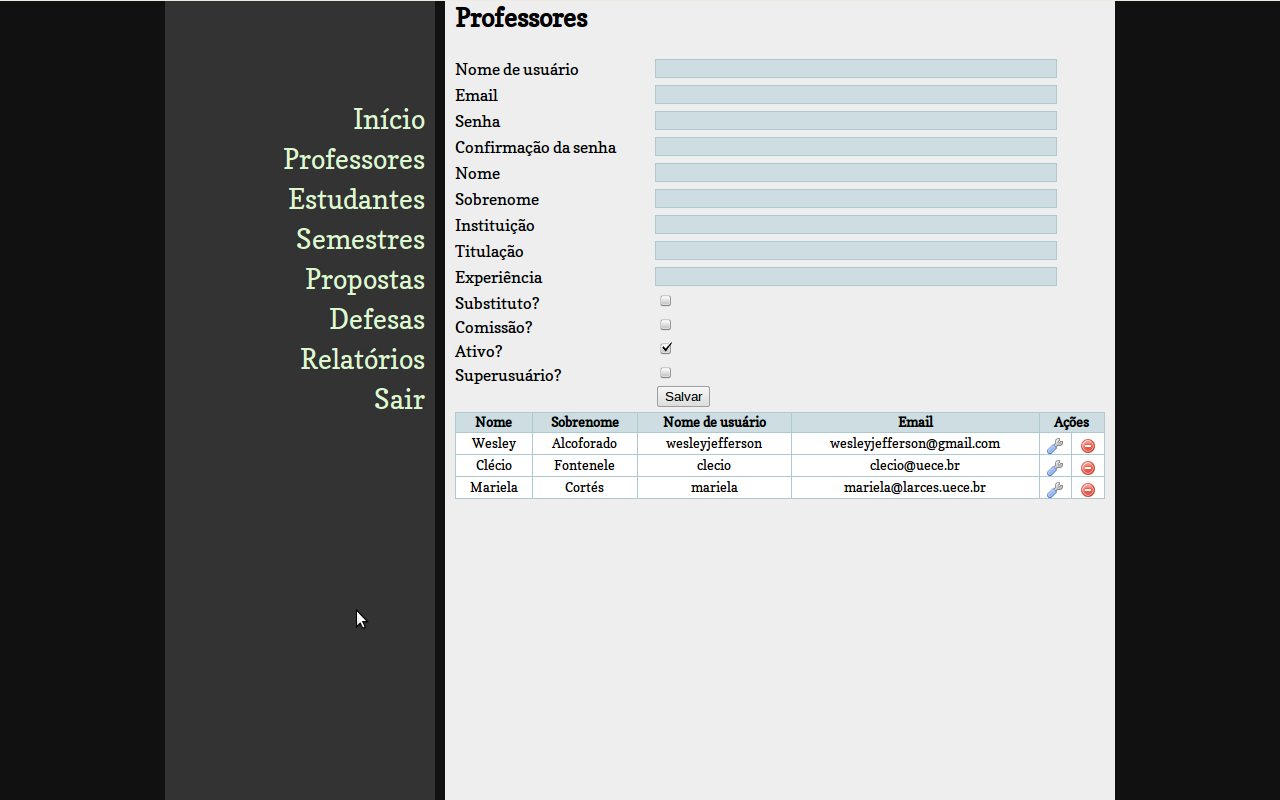
\includegraphics[width=1\textwidth]{fig/telas/administrador/crud_professor_listagem_pos_insercao.png}
\caption{Tela de cadastro de professores após a inserção de um professor}
\label{fig:crud_professor_listagem_pos_insercao}
\end{figure}

\begin{figure}[htbp]
\centering
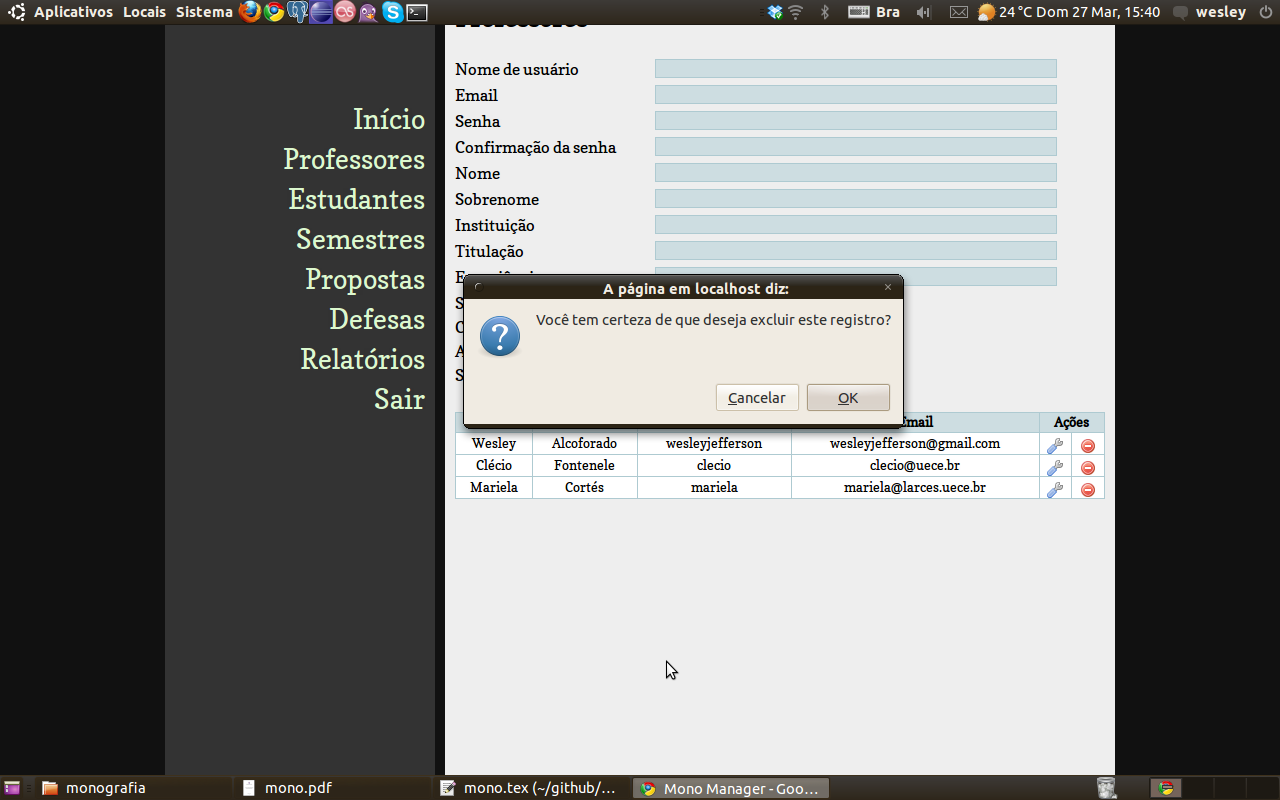
\includegraphics[width=1\textwidth]{fig/telas/administrador/crud_professor_remocao.png}
\caption{Confirmação de remoção de um professor}
\label{fig:crud_professor_remocao}
\end{figure}

Na Figura ~\ref{fig:crud_professor_insercao} mostra a tela de cadastro de professores, que
é acessada ao clicar na opção Professor no menu do sistema. Podemos ver que na tela
já se encontram disponíveis o formulário de edição e a listagem de todos os professores cadastrados 
no sistema. Na coluna Ações, na listagem de professores, estão disponíveis as ações de edição
e remoção de registro. A Figura ~\ref{fig:crud_professor_insercao} exibe o formulário sendo preenchido
para a inserção de um novo professor, ao passo que a Figura ~\ref{fig:crud_professor_listagem_pos_insercao}
exibe a listagem atualizada após a inserção de um novo professor no sistema. Se o administrador 
clicar no ícone de remoção de registro, uma janela de confirmação é exibida para que
o administrador confirme seu desejo de remoção do registro, visto que esta ação não pode
ser revertida. Este processo pode ser visualizado na Figura ~\ref{fig:crud_professor_remocao}.

\begin{figure}[htbp]
\centering
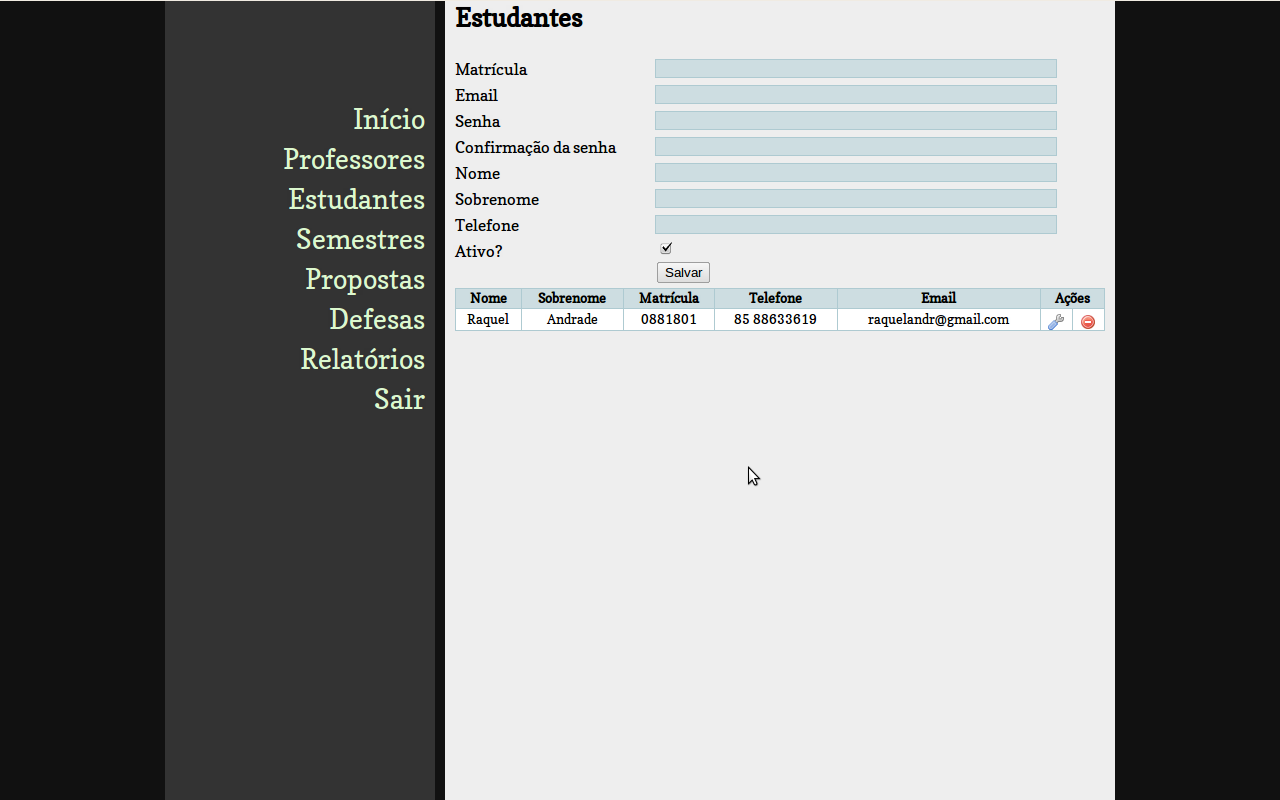
\includegraphics[width=1\textwidth]{fig/telas/administrador/crud_estudante.png}
\caption{Tela de cadastro de estudantes}
\label{fig:crud_estudante}
\end{figure}

A Figura ~\ref{fig:crud_estudante} exibe a tela de cadastro de estudantes. O mecanismo de funcionamento
desta é exatamente igual ao de cadastro de professores, portanto não há necessidade de mais detalhes.

\begin{figure}[htbp]
\centering
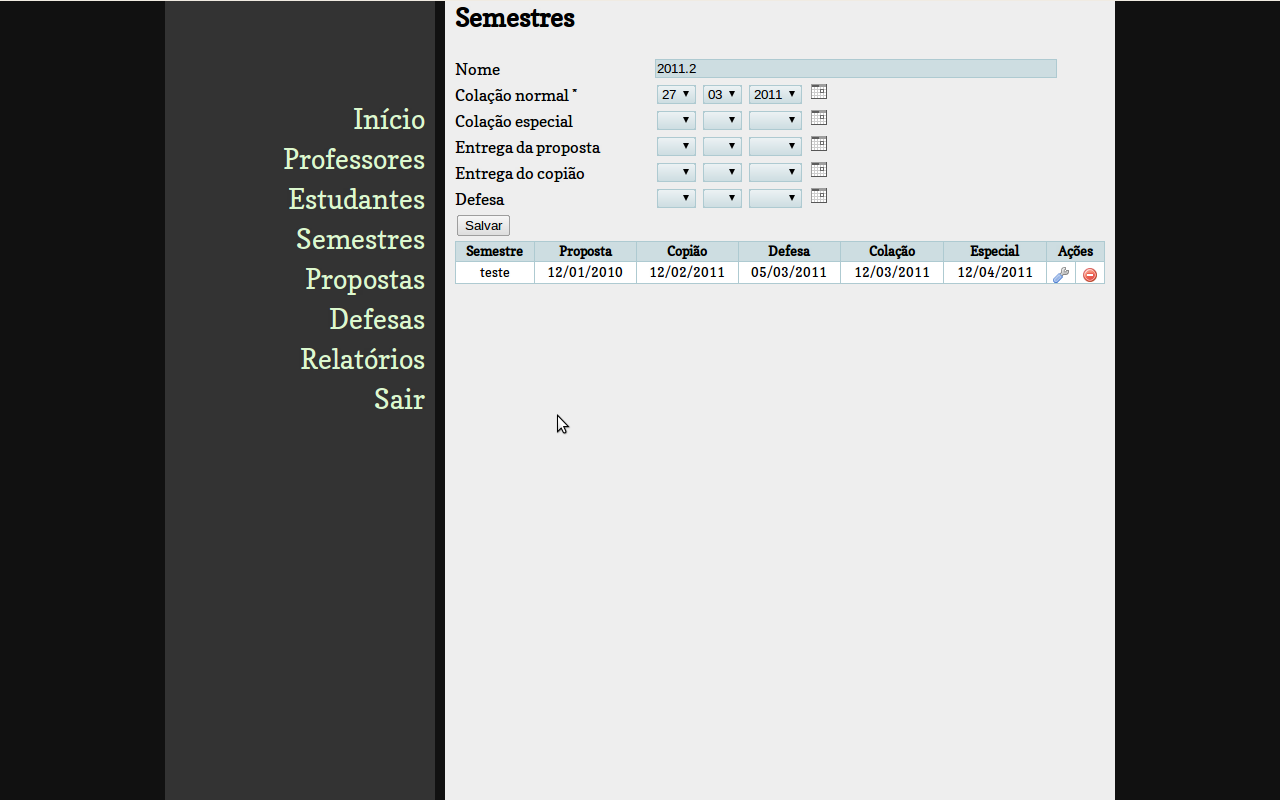
\includegraphics[width=1\textwidth]{fig/telas/administrador/crud_semestre.png}
\caption{Tela de cadastro de semestres}
\label{fig:crud_semestre}
\end{figure}

\begin{figure}[htbp]
\centering
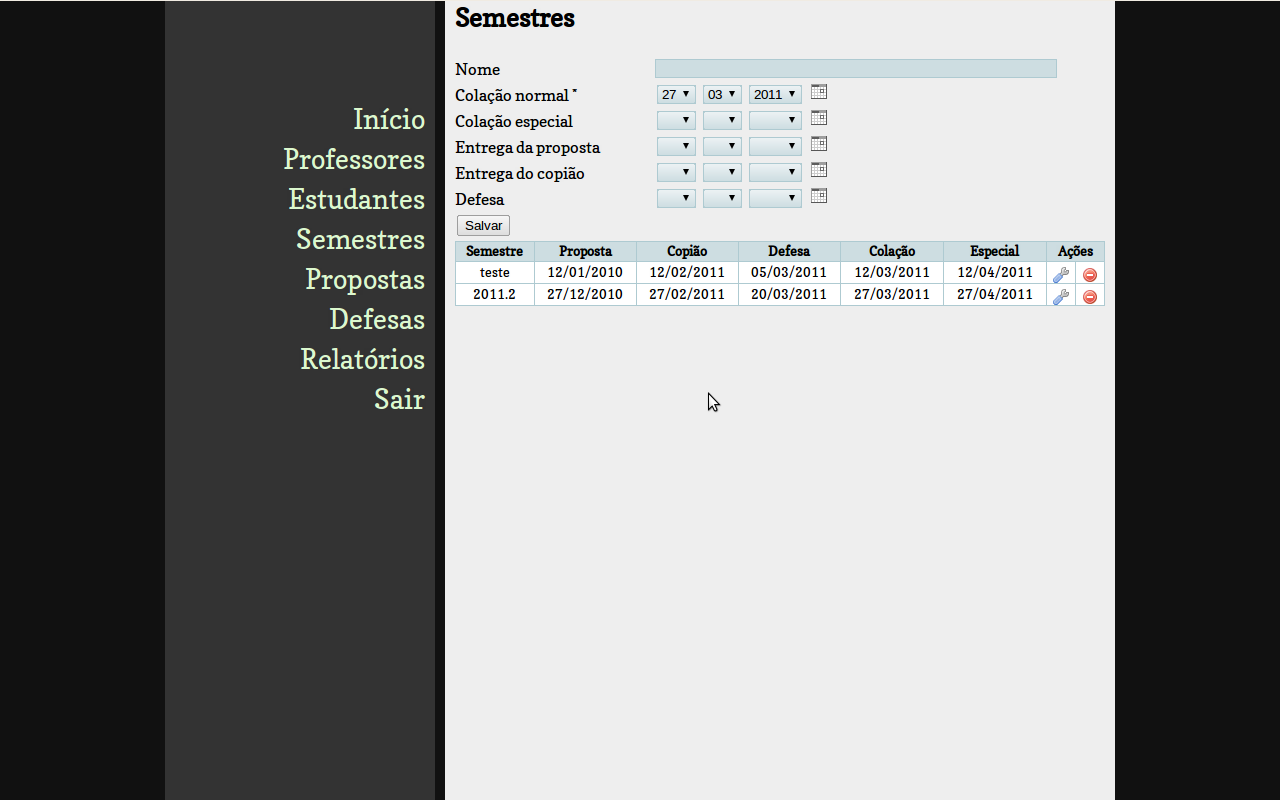
\includegraphics[width=1\textwidth]{fig/telas/administrador/crud_semestre_calculo_datas.png}
\caption{Tela de cadastro de semestres após o cadastro de um novo item}
\label{fig:crud_semestre_calculo_datas}
\end{figure}

A Figura ~\ref{fig:crud_semestre} mostra a tela de cadastro de semestres. Esta possui um funcionamento
muito parecido com o cadastro de professores e estudantes, porém possui uma particularidade que 
convém explicitar. O único campo obrigatório é a data de colação normal. A partir da informação desta
data, pode-se inferir todas as outras. O cálculo é feito a partir das informações estabelecidas
no regulamento da universidade, que pode ser conferido nas Seções ~\ref{sec:proposta} e ~\ref{sec:defesa}.
A Figura ~\ref{fig:crud_semestre_calculo_datas} exibe o item inserido no banco de dados com as
datas calculadas a partir da data de colação normal. Se por algum motivo as datas forem diferentes,
o administrador pode informá-las separadamente. O sistema só tenta calcular aquelas que não foram
informadas.

\begin{figure}[htbp]
\centering
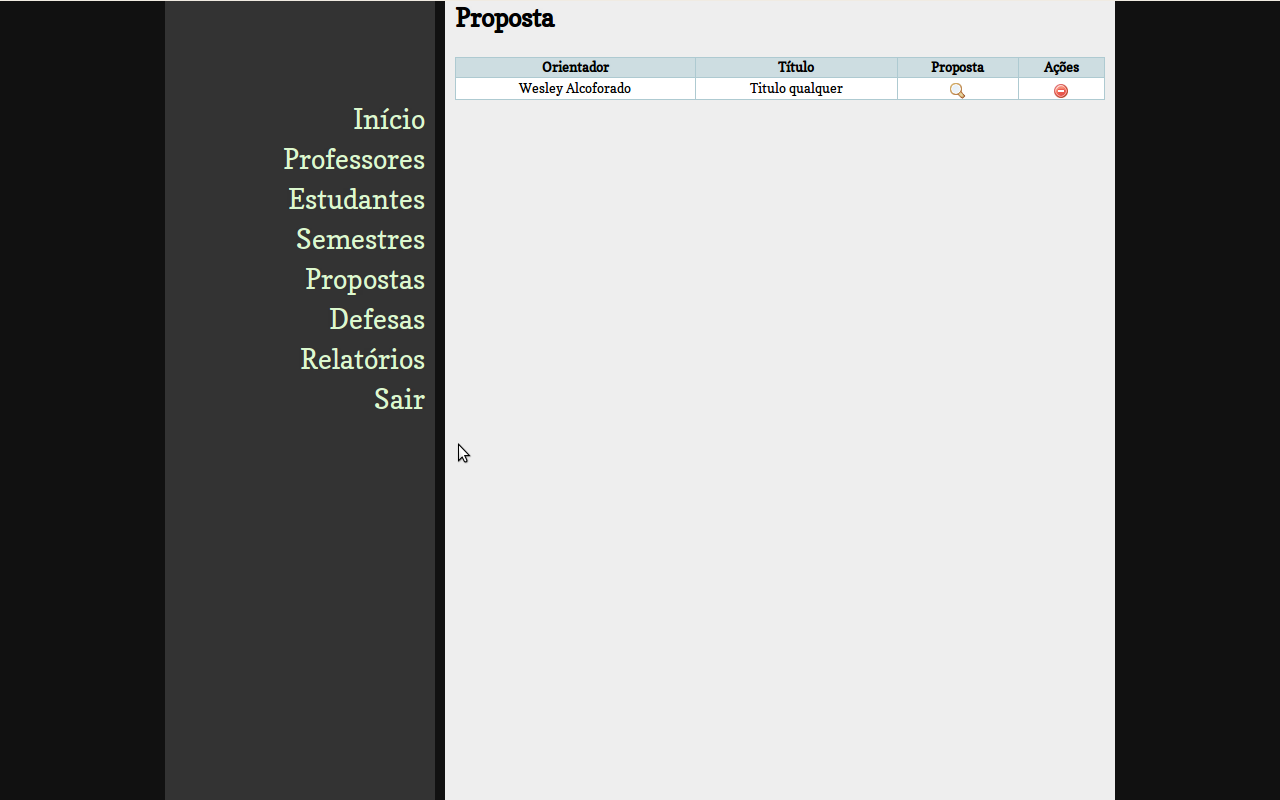
\includegraphics[width=1\textwidth]{fig/telas/administrador/propostas.png}
\caption{Tela de visualização de propostas no perfil do administrador}
\label{fig:propostas}
\end{figure}

\begin{figure}[htbp]
\centering
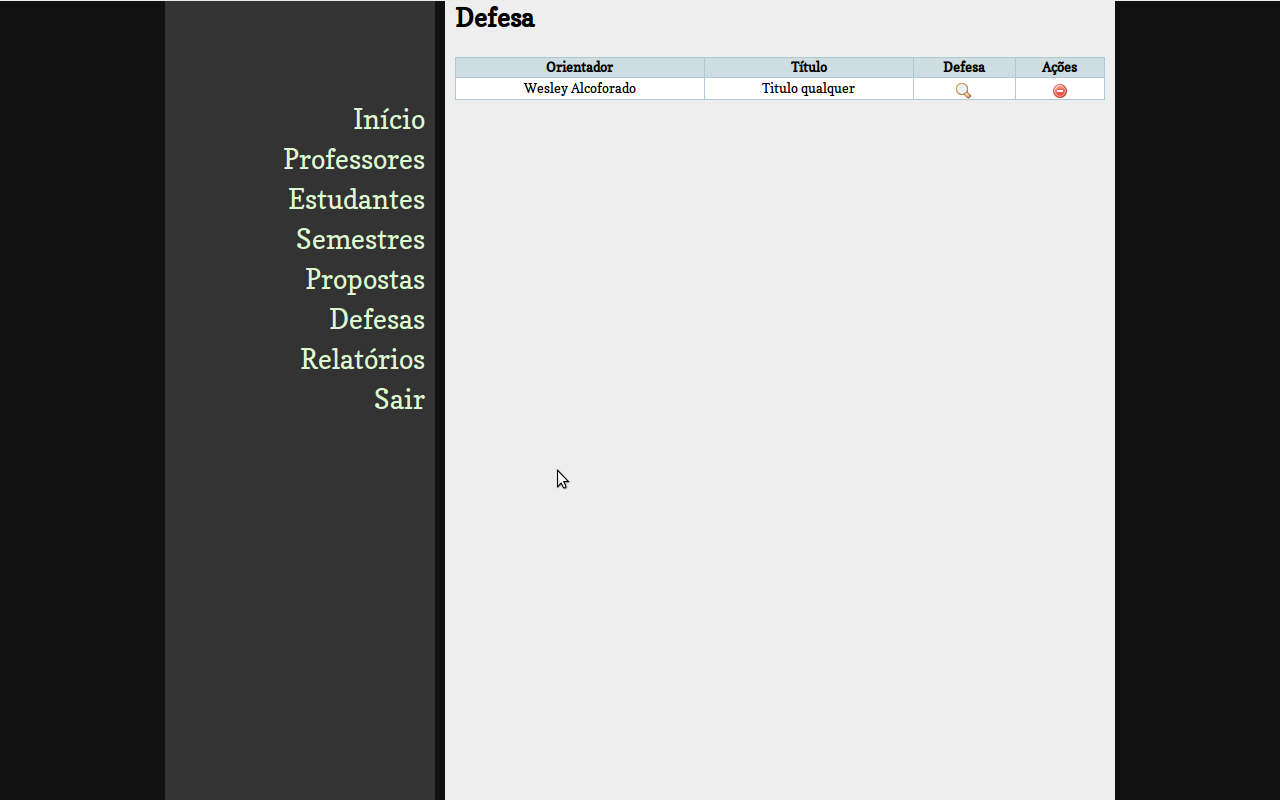
\includegraphics[width=1\textwidth]{fig/telas/administrador/defesas.png}
\caption{Tela de visualização de defesas no perfil do administrador}
\label{fig:defesas}
\end{figure}

\begin{figure}[htbp]
\centering
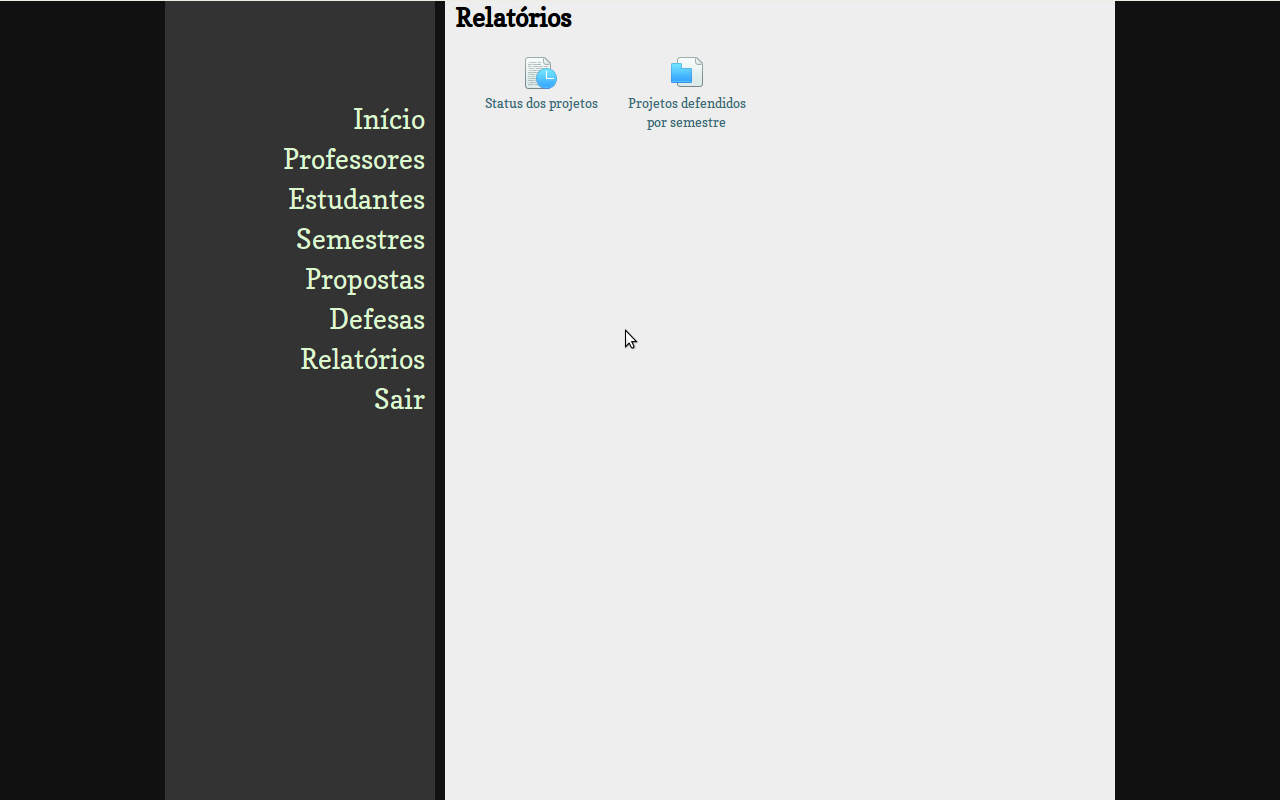
\includegraphics[width=1\textwidth]{fig/telas/administrador/relatorios.png}
\caption{Tela de consulta de relatórios}
\label{fig:relatorios}
\end{figure}

A Figura ~\ref{fig:propostas} exibe a tela de visualização de propostas e a Figura ~\ref{fig:defesas}
exibe a tela de visualização de defesas no perfil do administardor. Ambas possuem um ícone em formato
de lupa que permite visualizar a proposta do projeto ou o copião (no caso de uma solicitação de defesa), e
possuem um ícone para remover o registro do banco de dados. A Figura ~\ref{fig:relatorios} exibe a tela
de consulta de relatórios, que é compartilhada entre os perfis de administrador e comissão.

\subsection{Perfil de estudante}
O estudante só precisa se preocupar com o desenvolvimento do seu próprio projeto, por isso, o único
módulo que ele precisa ter acesso é o de projetos. A Figura ~\ref{fig:aluno_01_projeto_novo} exibe
o formulário de projetos sendo preenchido pelo estudante, onde ele só precisa informar o nome do
seu projeto e quem são seus orientadores. A Figura ~\ref{fig:aluno_02_projeto_cadastrado} exibe como fica
a listagem de projetos após a inserção do novo item. Podemos notar que quando o projeto é cadastrado, seu 
status indica que a proposta está pendente. A Figura ~\ref{fig:aluno_03_anexo_proposta} exibe a tela de anexo
de propostas, que pode ser acessada pelo ícone em formato de clipe na coluna Proposta. Após a anexação
da proposta (Figura ~\ref{fig:aluno_04_proposta_anexada}), um email é enviado ao orientador, informando-o
que um de seus alunos acabou de anexar uma proposta e que sua aprovação é necessária. O aluno
deve aguardar que o orientador e a comissão aprovem sua proposta para iniciar o desenvolvimento do
trabalho. Quando isso acontecer, o estudante deverá receber um email notificando a novidade.
As Figuras ~\ref{fig:aluno_05_proposta_aprovada_orientador} e ~\ref{fig:aluno_06_proposta_aprovada_comissao}
demonstram as modificações do status do projeto à medida que o orientador e a comissão avaliam 
a sua proposta.

A partir da tela da Figura ~\ref{fig:aluno_06_proposta_aprovada_comissao}, o ícone em formato de apresentação
de slides fica disponível para o estudante, significando que ele pode submeter uma solicitação de defesa. Ao
clicar no ícone, a tela da Figura ~\ref{fig:aluno_07_submetendo_defesa} é carregada, solicitando ao
estudante os itens necessários para a solicitação da defesa, como o documento do copião.

As Figuras ~\ref{fig:aluno_08_defesa_nao_analisada}, ~\ref{fig:aluno_09_defesa_analisada_professor}, 
~\ref{fig:aluno_10_defesa_analisada_comissao} e ~\ref{fig:aluno_11_projeto_defendido} mostram 
respectivamente a evolução do status do projeto à medida em que o estudante solicita
a defesa, o orientador a aprova, a comissão a aprova e a comissão identifica que a defesa foi efetivamente concluida.


\begin{figure}[htbp]
\centering
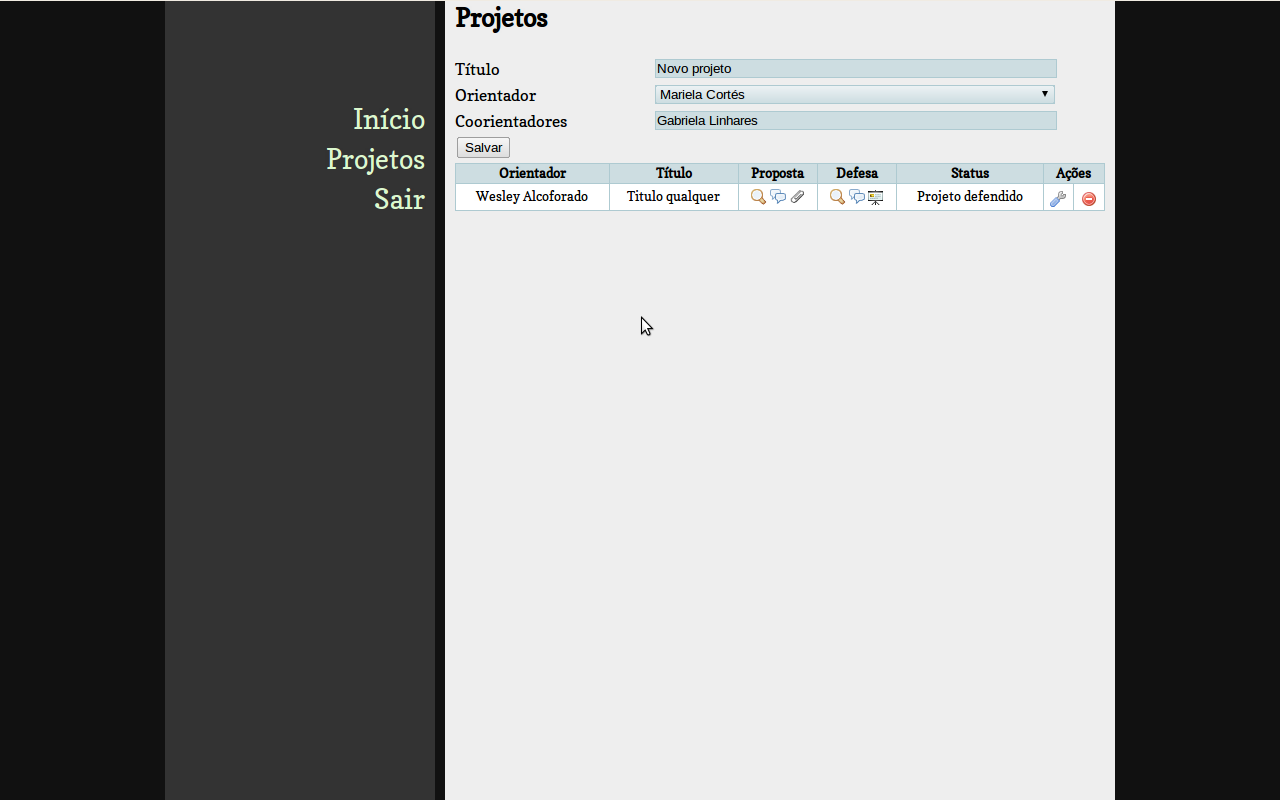
\includegraphics[width=1\textwidth]{fig/telas/processo/aluno_01_projeto_novo.png}
\caption{Tela de cadastro de projetos}
\label{fig:aluno_01_projeto_novo}
\end{figure}

\begin{figure}[htbp]
\centering
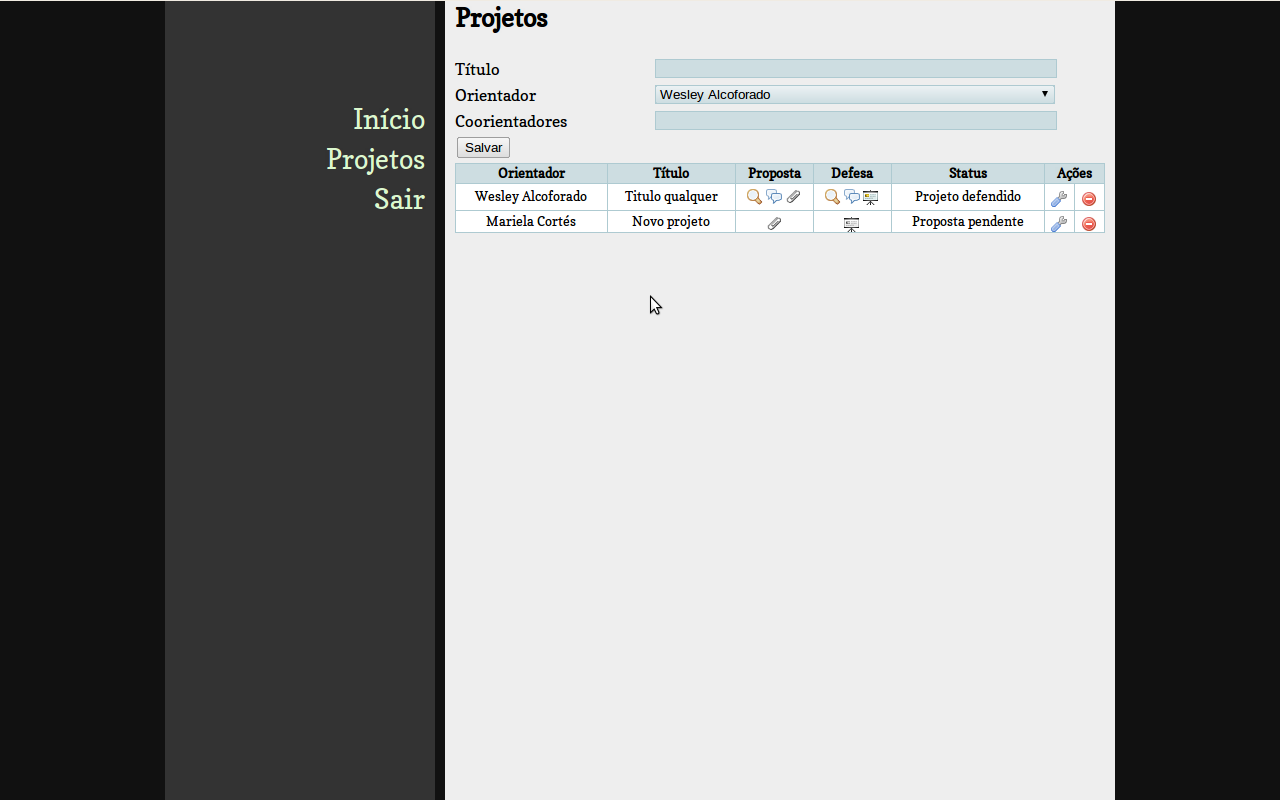
\includegraphics[width=1\textwidth]{fig/telas/processo/aluno_02_projeto_cadastrado.png}
\caption{Tela de cadastro de projetos após a inserção de novo item}
\label{fig:aluno_02_projeto_cadastrado}
\end{figure}

\begin{figure}[htbp]
\centering
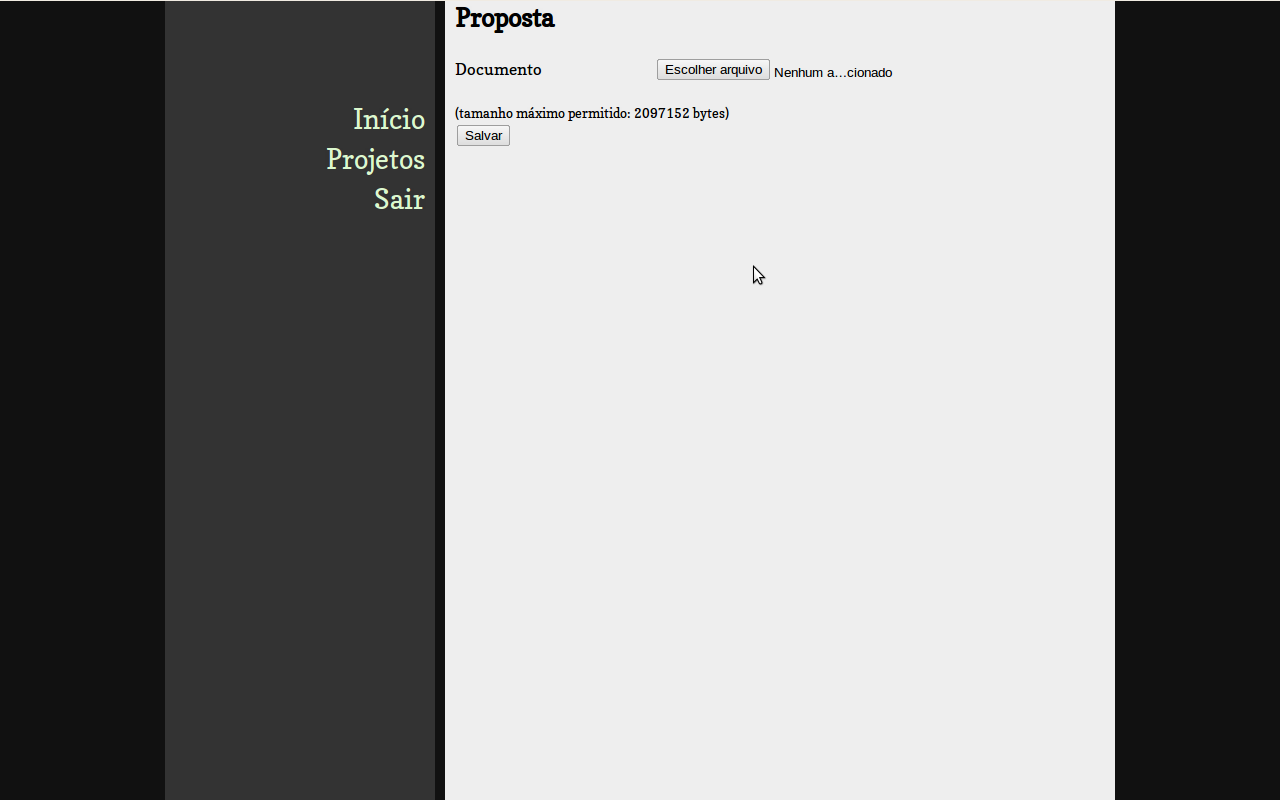
\includegraphics[width=1\textwidth]{fig/telas/processo/aluno_03_anexo_proposta.png}
\caption{Tela de anexo de propostas}
\label{fig:aluno_03_anexo_proposta}
\end{figure}

\begin{figure}[htbp]
\centering
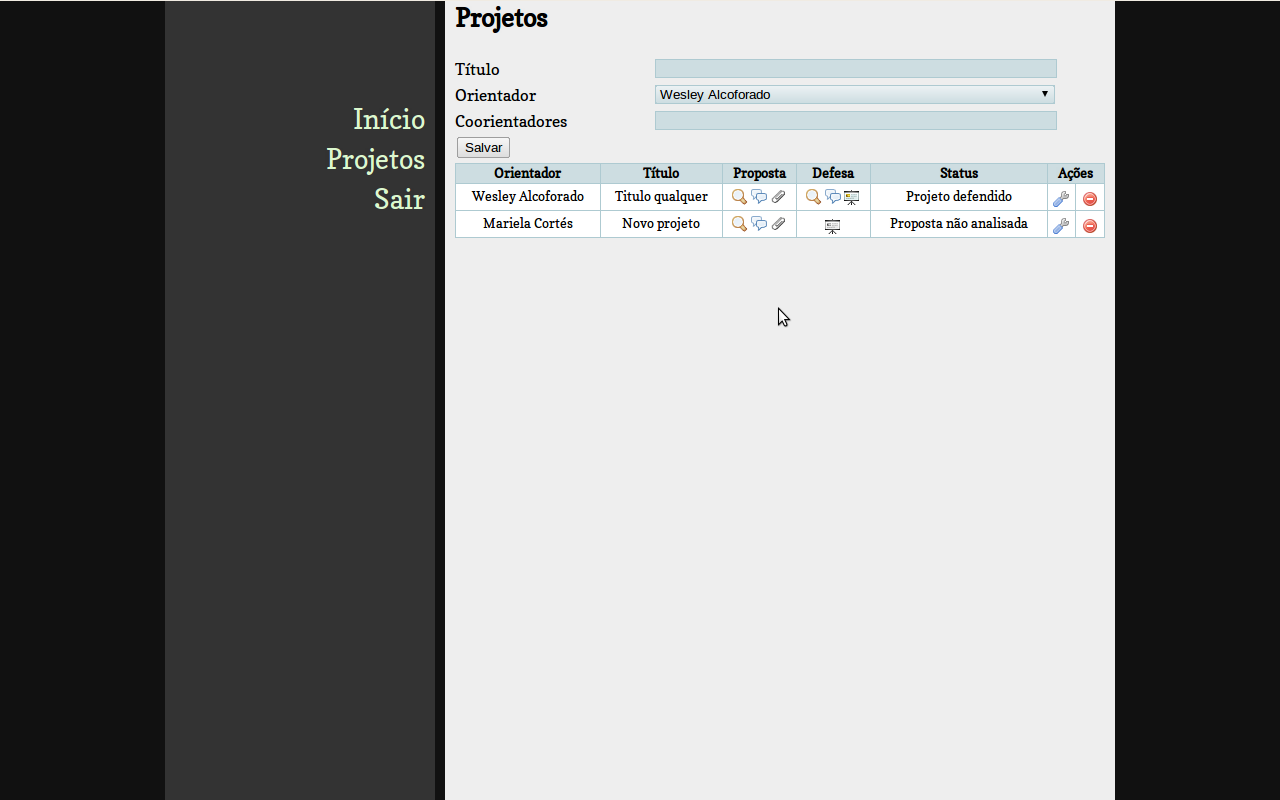
\includegraphics[width=1\textwidth]{fig/telas/processo/aluno_04_proposta_anexada.png}
\caption{Tela de cadastro de projetos após a anexação de uma proposta}
\label{fig:aluno_04_proposta_anexada}
\end{figure}

\begin{figure}[htbp]
\centering
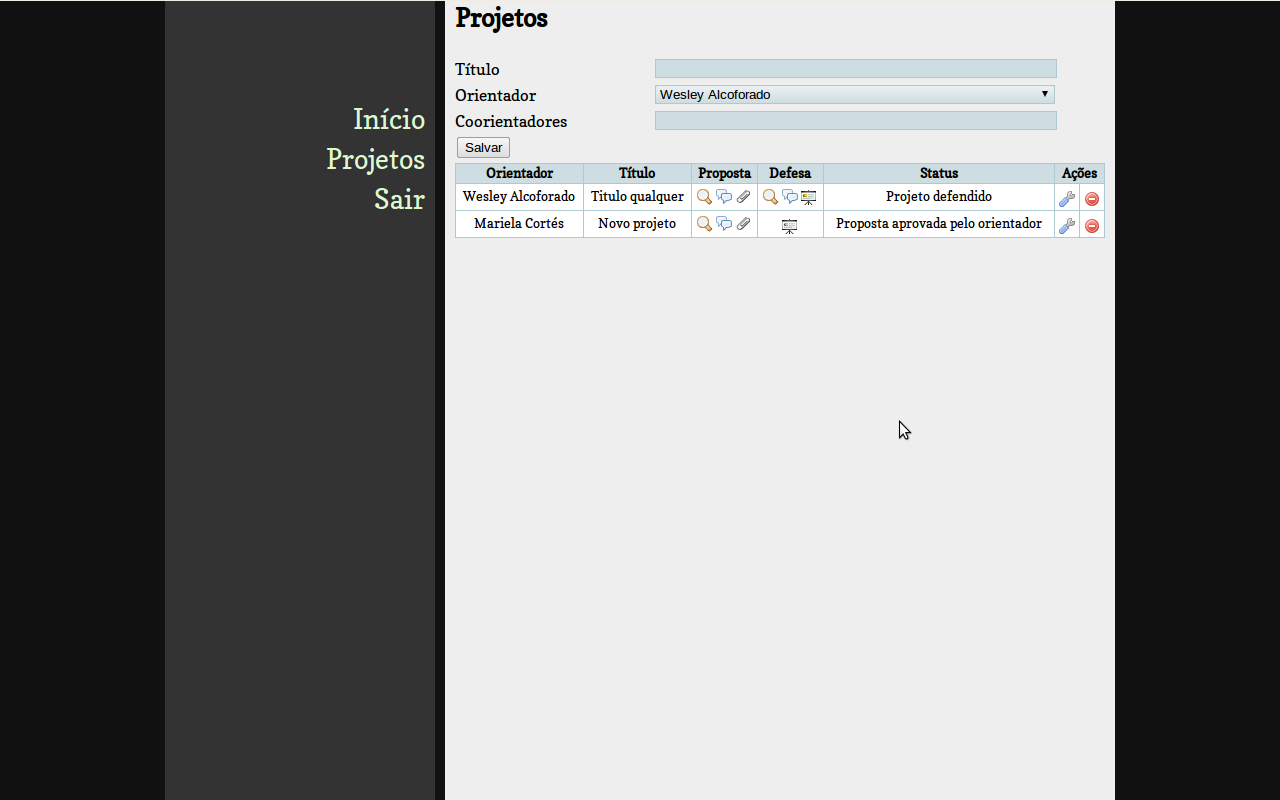
\includegraphics[width=1\textwidth]{fig/telas/processo/aluno_05_proposta_aprovada_orientador.png}
\caption{Tela de cadastro de projetos após a aprovação do orientador}
\label{fig:aluno_05_proposta_aprovada_orientador}
\end{figure}

\begin{figure}[htbp]
\centering
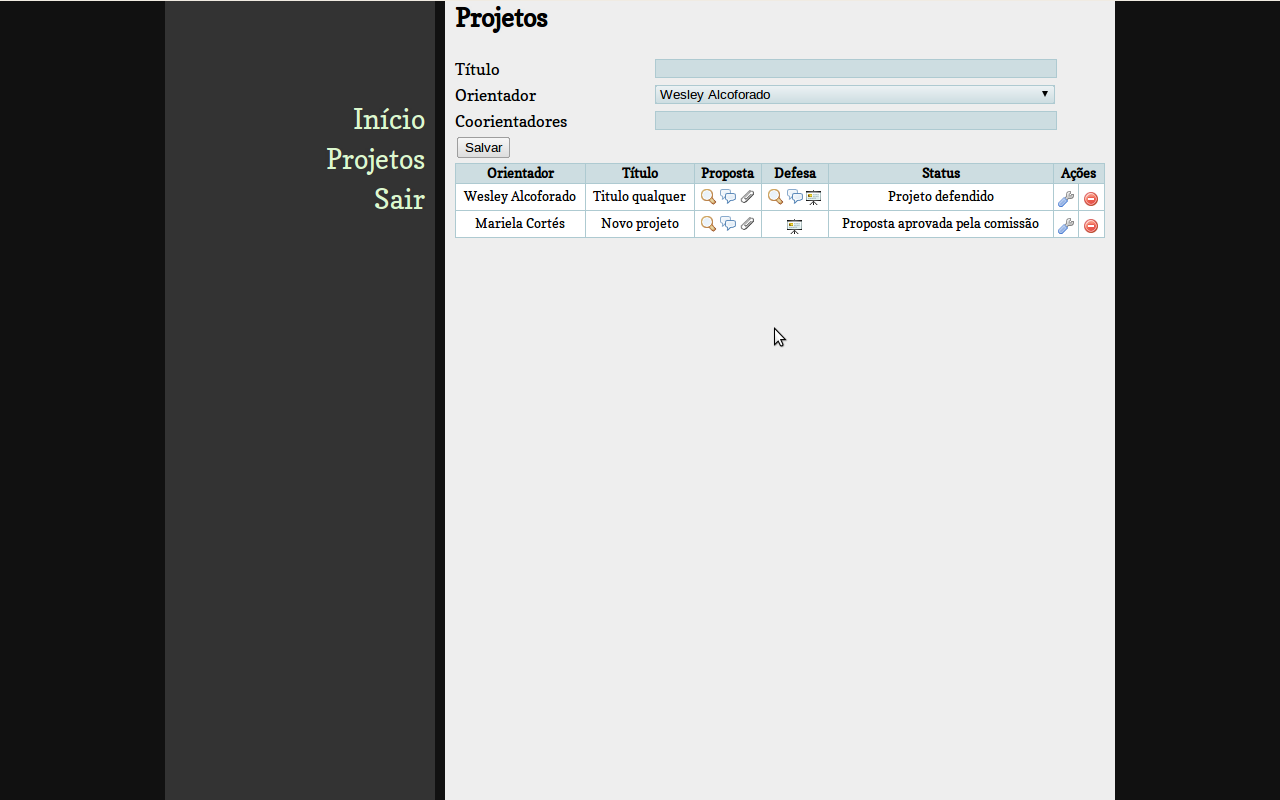
\includegraphics[width=1\textwidth]{fig/telas/processo/aluno_06_proposta_aprovada_comissao.png}
\caption{Tela de cadastro de projetos após a aprovação da comissão}
\label{fig:aluno_06_proposta_aprovada_comissao}
\end{figure}

\begin{figure}[htbp]
\centering
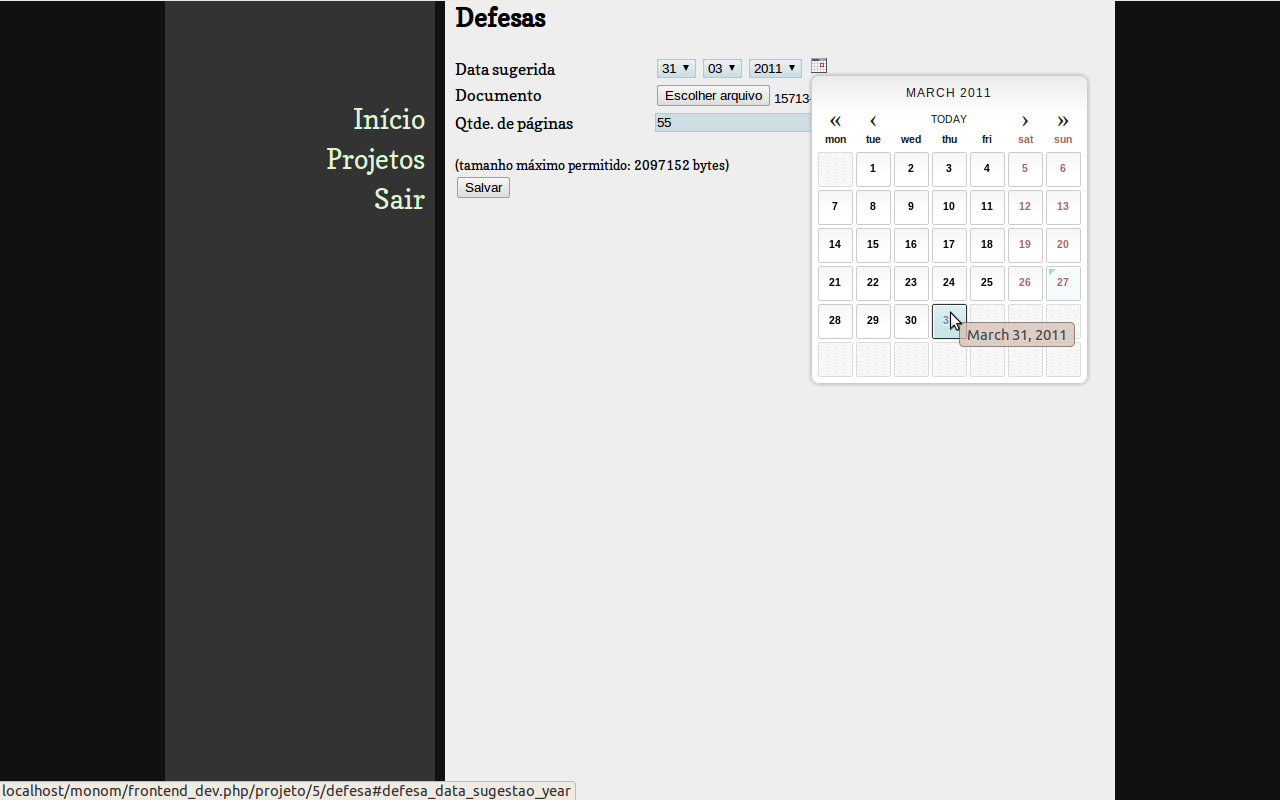
\includegraphics[width=1\textwidth]{fig/telas/processo/aluno_07_submetendo_defesa.png}
\caption{Tela de solicitação de defesa}
\label{fig:aluno_07_submetendo_defesa}
\end{figure}

\begin{figure}[htbp]
\centering
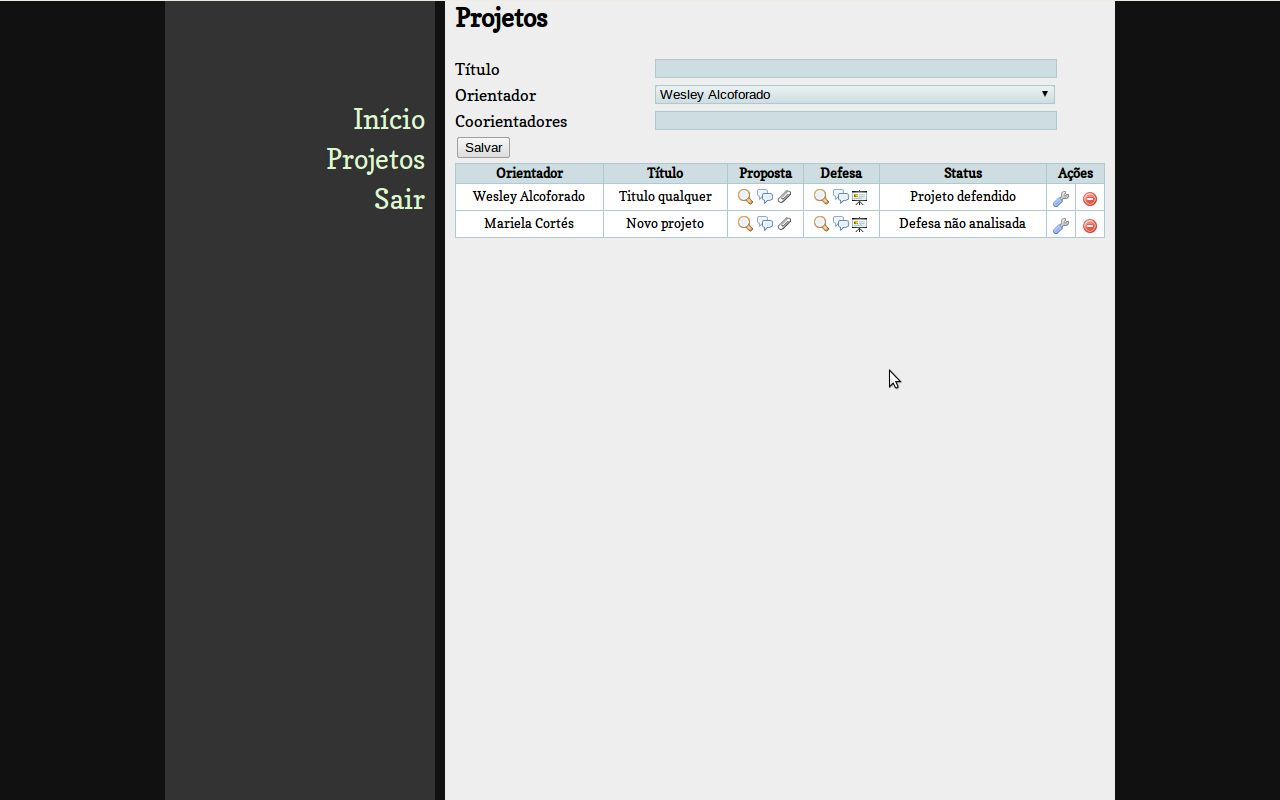
\includegraphics[width=1\textwidth]{fig/telas/processo/aluno_08_defesa_nao_analisada.png}
\caption{Tela de cadastro de projetos após a solicitação de defesa}
\label{fig:aluno_08_defesa_nao_analisada}
\end{figure}

\begin{figure}[htbp]
\centering
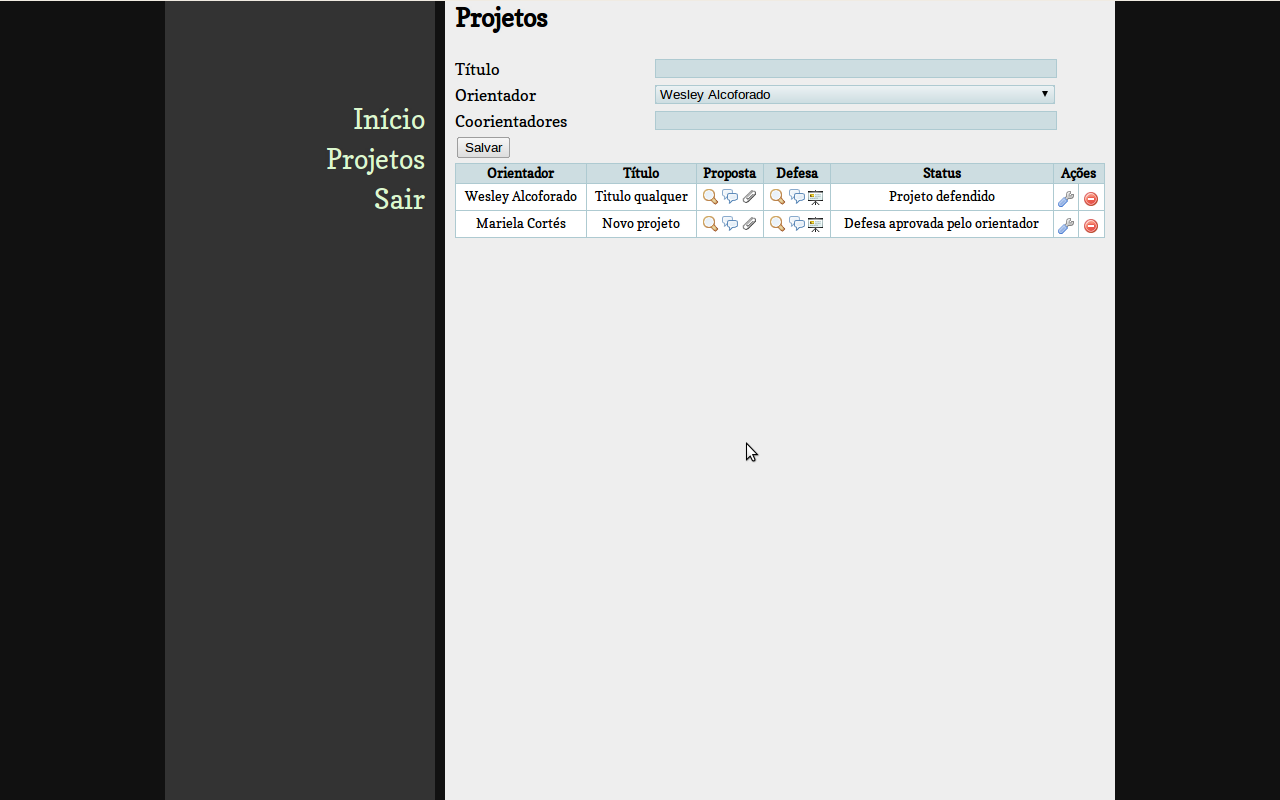
\includegraphics[width=1\textwidth]{fig/telas/processo/aluno_09_defesa_analisada_professor.png}
\caption{Tela de cadastro de projetos após a aprovação do orientador}
\label{fig:aluno_09_defesa_analisada_professor}
\end{figure}

\begin{figure}[htbp]
\centering
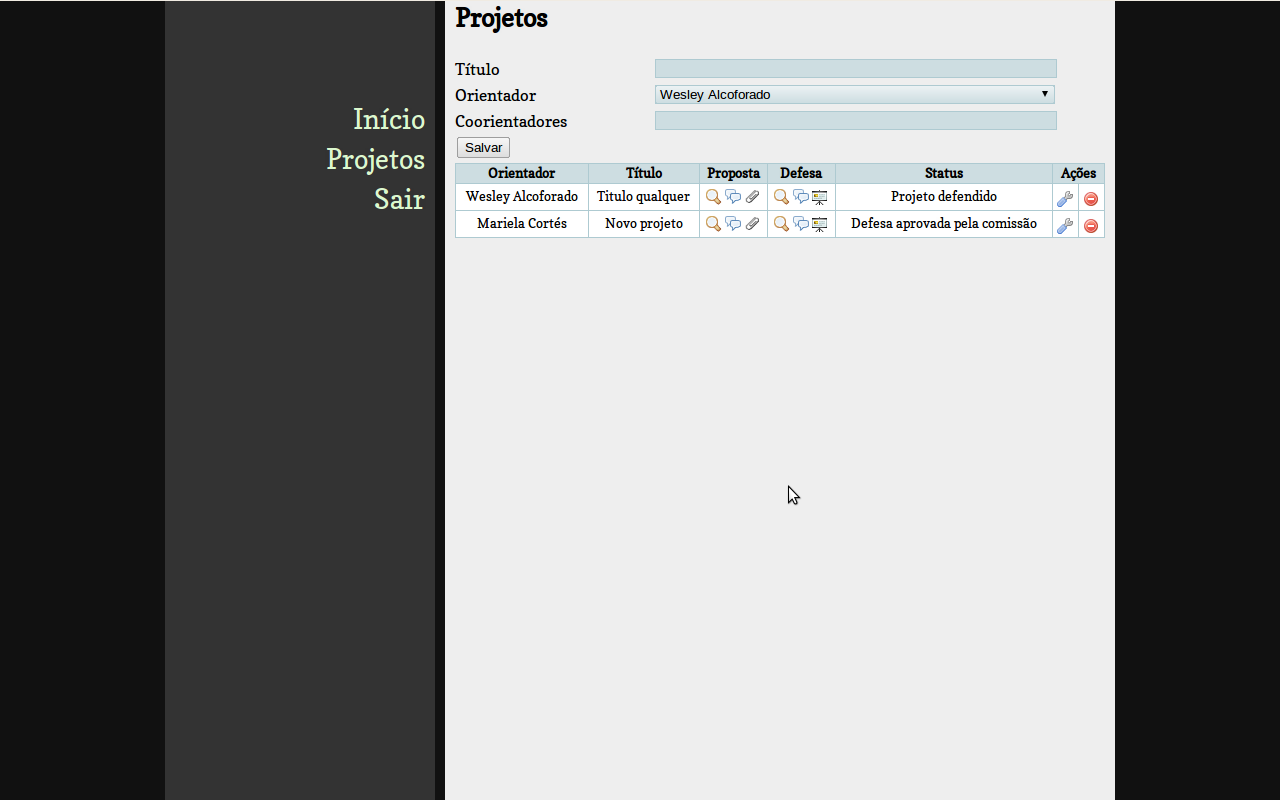
\includegraphics[width=1\textwidth]{fig/telas/processo/aluno_10_defesa_analisada_comissao.png}
\caption{Tela de cadastro de projetos após a aprovação da comissão}
\label{fig:aluno_10_defesa_analisada_comissao}
\end{figure}

\begin{figure}[htbp]
\centering
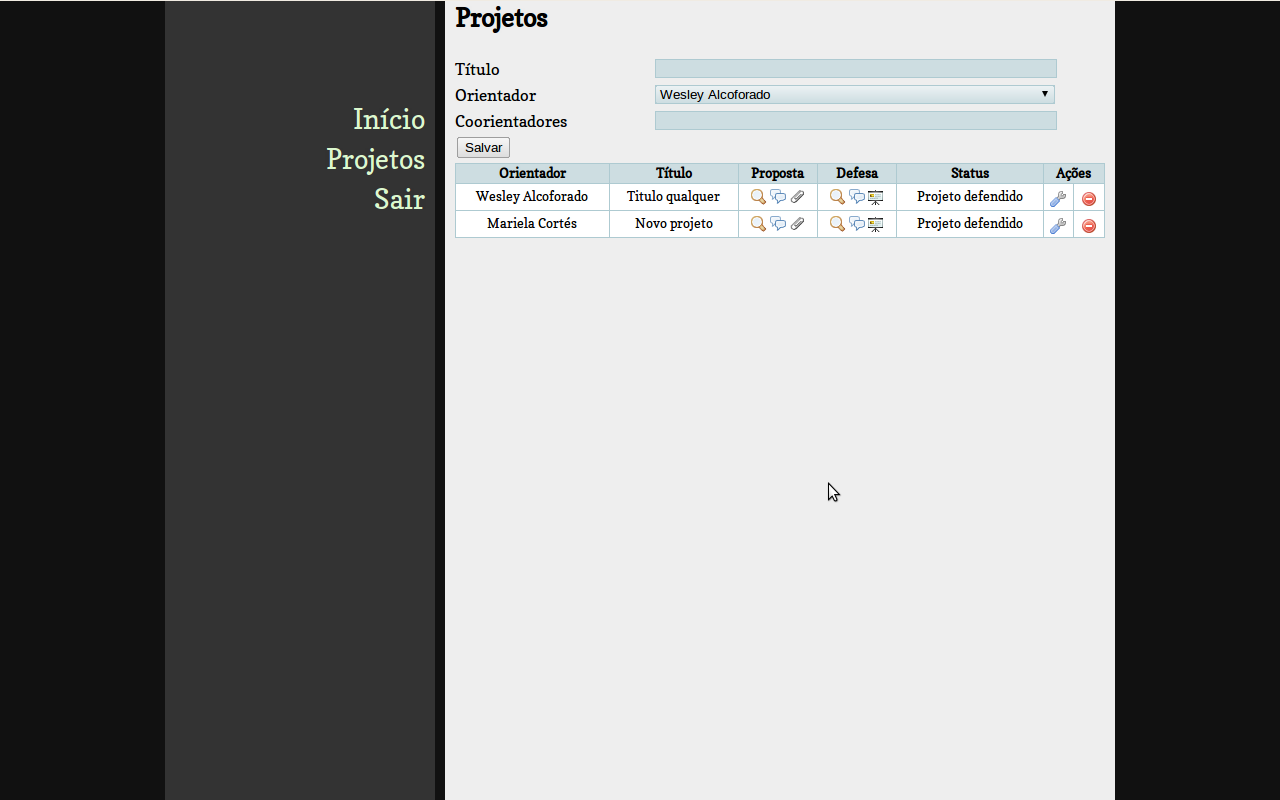
\includegraphics[width=1\textwidth]{fig/telas/processo/aluno_11_projeto_defendido.png}
\caption{Tela de cadastro de projetos após a comissão ter indicado que a defesa foi concluida}
\label{fig:aluno_11_projeto_defendido}
\end{figure}

\subsection{Perfil de professor (orientador)}
O orientador possui acesso aos projetos de seus orientandos, e deve dar o seu aval para quaisquer 
submissões que o estudante envie para a comissão de projeto final.

A Figura ~\ref{fig:professor_01_aprovacao proposta} exibe a tela de listagem de propostas
enviadas pelos orientandos. Propostas ainda não avaliadas pelo professor aparecem com dois ícones
de polegar para cima e polegar para baixo, que indicam que o professor aprova ou não a proposta, respectivamente.
Se o professor clicar no ícone em formato de lupa, ele pode visualizar o documento associado ao pedido.

A Figura ~\ref{fig:professor_02_prosta_sendo_aprovada} mostra o momento em que o professor
clica na opção de aprovar a proposta e a Figura ~\ref{fig:professor_03_proposta_aprovada} o momento
seguinte a esta ação.

Para o perfil de professor, o módulo de Defesas é completamente idêntico ao módulo de propostas, o que
podemos perceber pela Figura ~\ref{fig:professor_04_avaliando_defesa}.

\begin{figure}[htbp]
\centering
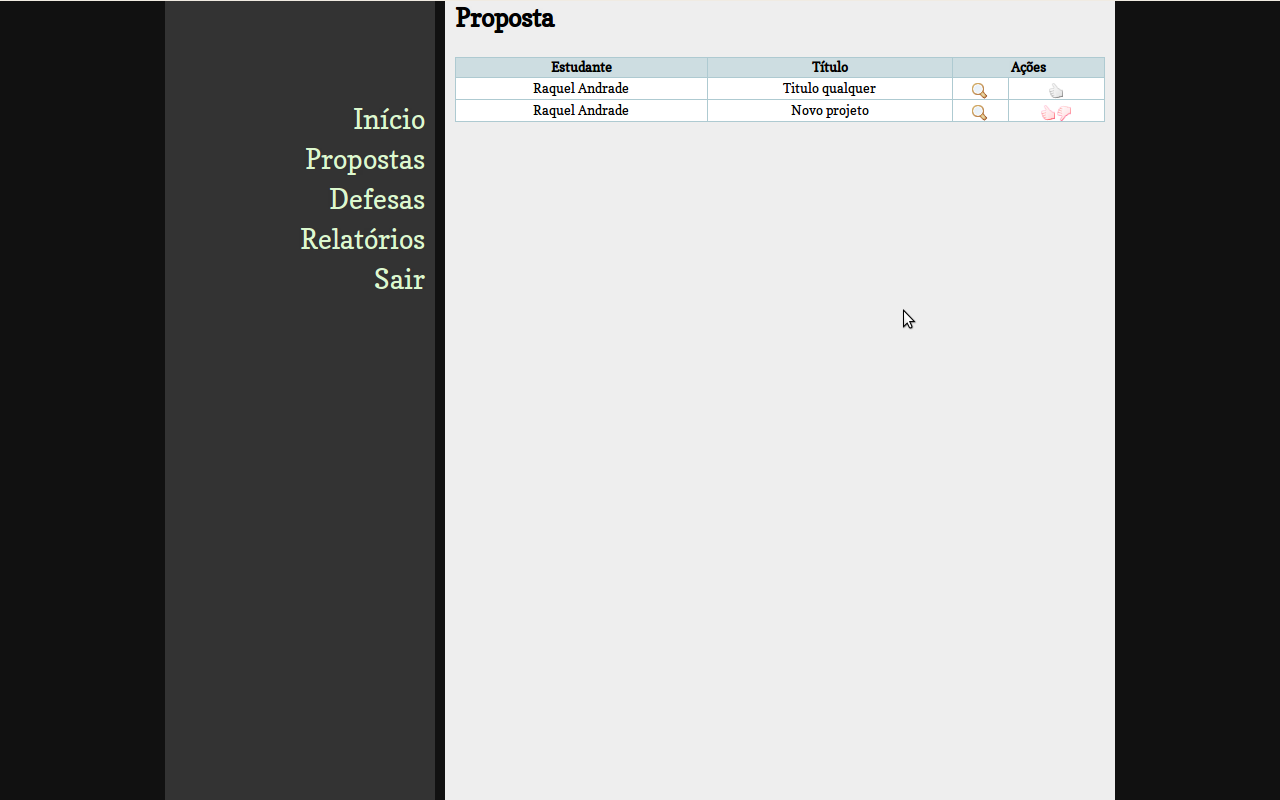
\includegraphics[width=1\textwidth]{fig/telas/processo/professor_01_aprovacao proposta.png}
\caption{Tela de listagem de propostas submetidas pelos orientandos}
\label{fig:professor_01_aprovacao proposta}
\end{figure}

\begin{figure}[htbp]
\centering
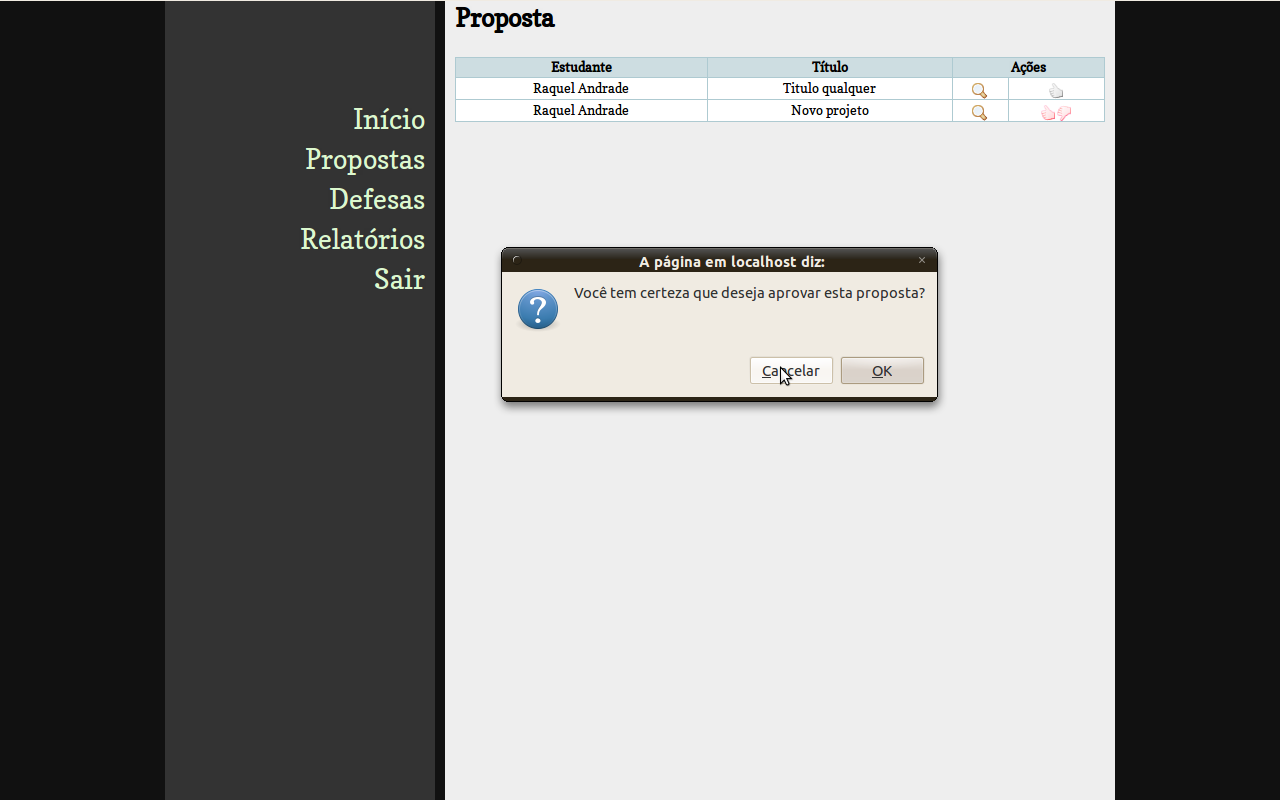
\includegraphics[width=1\textwidth]{fig/telas/processo/professor_02_prosta_sendo_aprovada.png}
\caption{Proposta sendo aprovada pelo orientador}
\label{fig:professor_02_prosta_sendo_aprovada}
\end{figure}

\begin{figure}[htbp]
\centering
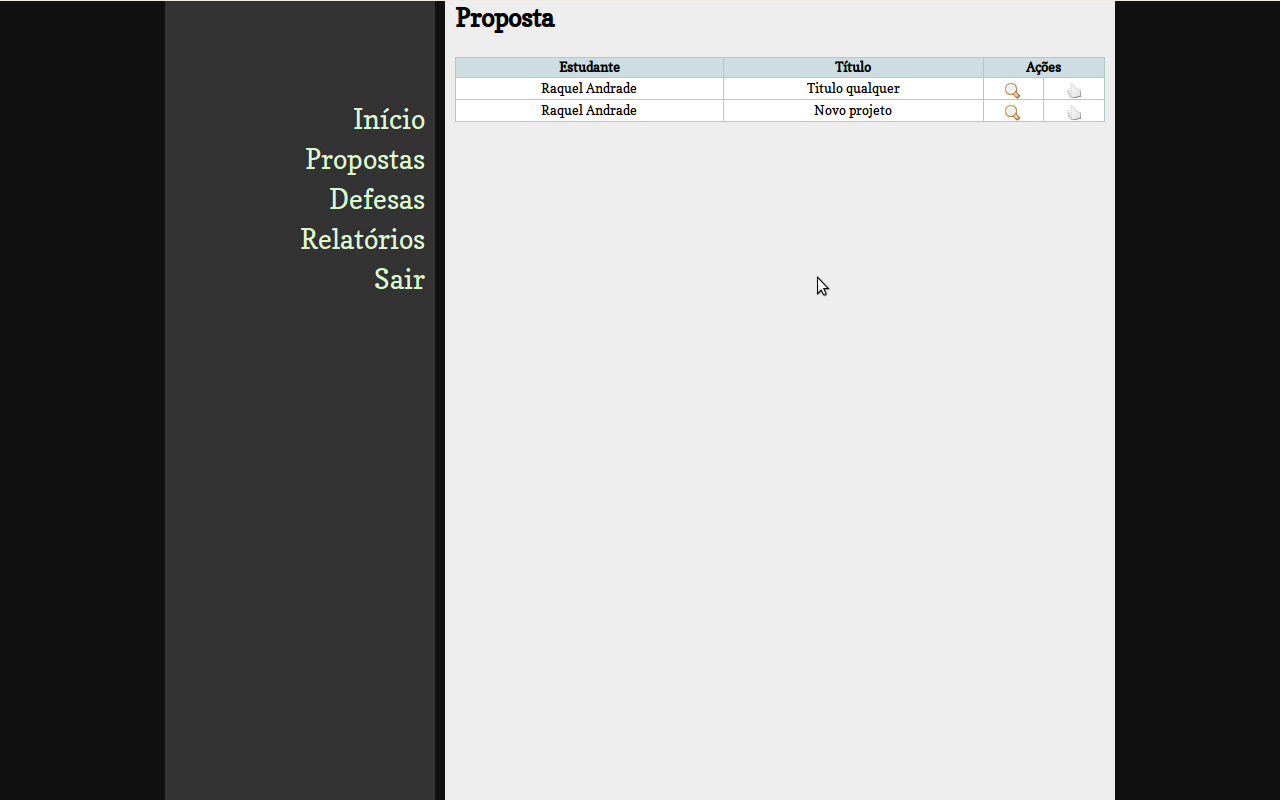
\includegraphics[width=1\textwidth]{fig/telas/processo/professor_03_proposta_aprovada.png}
\caption{Tela de listagem de propostas após o orientador ter aprovado uma proposta}
\label{fig:professor_03_proposta_aprovada}
\end{figure}

\begin{figure}[htbp]
\centering
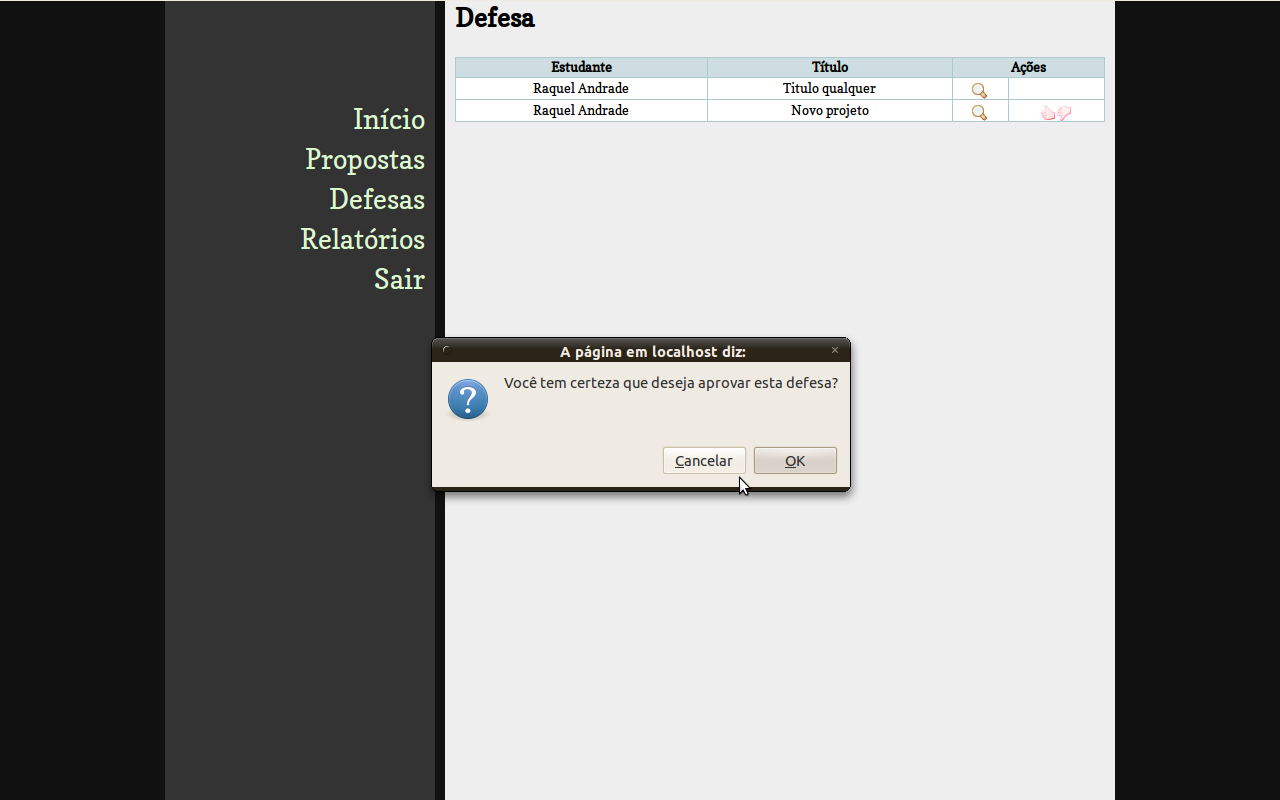
\includegraphics[width=1\textwidth]{fig/telas/processo/professor_04_avaliando_defesa.png}
\caption{Tela de listagem de requisições de defesa submetidas pelos orientandos}
\label{fig:professor_04_avaliando_defesa}
\end{figure}

\subsection{Perfil de comissão}
A comissão precisa dar o parecer final em qualquer submissão feito pelo estudante. É ela quem
decide se uma proposta de projeto pode ser desenvolvida ou não, da mesma forma que é ela quem
decide se o estudante já pode defender seu projeto.

A Figura ~\ref{fig:comissao_01_propostas} exibe a tela de listagem de propostas e uma coluna de
ações. Na primeira subcoluna, há um ícone em formato de lupa que permite à comissão visualizar
o documento da proposta anexada. O segundo ícone, em formato de balões de conversação permite
a um integrante da comissão saber quais foram os comentários feitos pelos outros integrantes sobre
a proposta em questão. O último ícone assume o formato de martelo de decisão quando a proposta
ainda não foi analisada e assume o formato de polegar para cima ou para baixo dependendo da 
avaliação final. Ao clicar no ícone do martelo, a tela da Figura ~\ref{fig:comissao_02_proposta_sendo_avaliada}
é exibida, permitindo ao integrante da comissão dar seu parecer e fornecer um comentário opcional
sobre a proposta. Uma tela de confirmação é exibida quando o integrante seleciona as opções Aprovar
ou Desaprovar, como pode ser observado na mesma figura.

A Figura ~\ref{fig:comissao_03_proposta_avaliada} exibe o status da listagem após a aprovação da
proposta e a Figura ~\ref{fig:comissao_04_comentarios} exibe a tela de comentários, que surge
após o integrante da comissão clicar no ícone em formato de balões de conversação. 

Para a avaliação das solicitações de defesa, o esquema é idêntico ao das propostas, como pode
ser observado na Figura ~\ref{fig:comissao_05_aprovando_defesa}. Existe uma pequena diferença
no ícone do martelo de decisão após a comissão aprovar a solicitação de defesa, como pode ser visto
na Figura ~\ref{fig:comissao_06_marcando_projeto_como_defendido}: o ícone é substituido por um
marcador verde, que deve ser clicado para que a comissão possa confirmar que o estudante
efetivamente defendeu o TCC e todo o seu processo foi concluido. Após a marcação deste ícone,
ele fica cinza e desabilitado.

\begin{figure}[htbp]
\centering
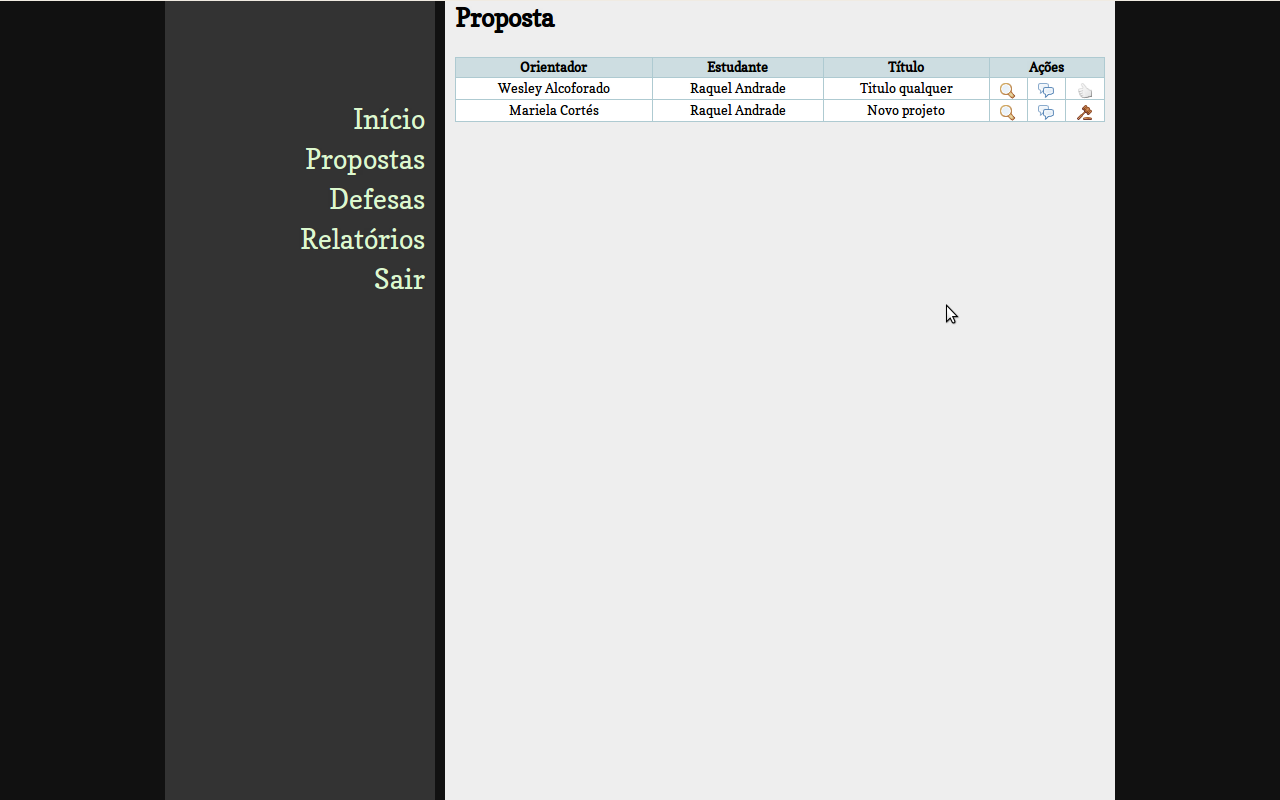
\includegraphics[width=1\textwidth]{fig/telas/processo/comissao_01_propostas.png}
\caption{Tela de listagem de propostas no perfil da comissão}
\label{fig:comissao_01_propostas}
\end{figure}

\begin{figure}[htbp]
\centering
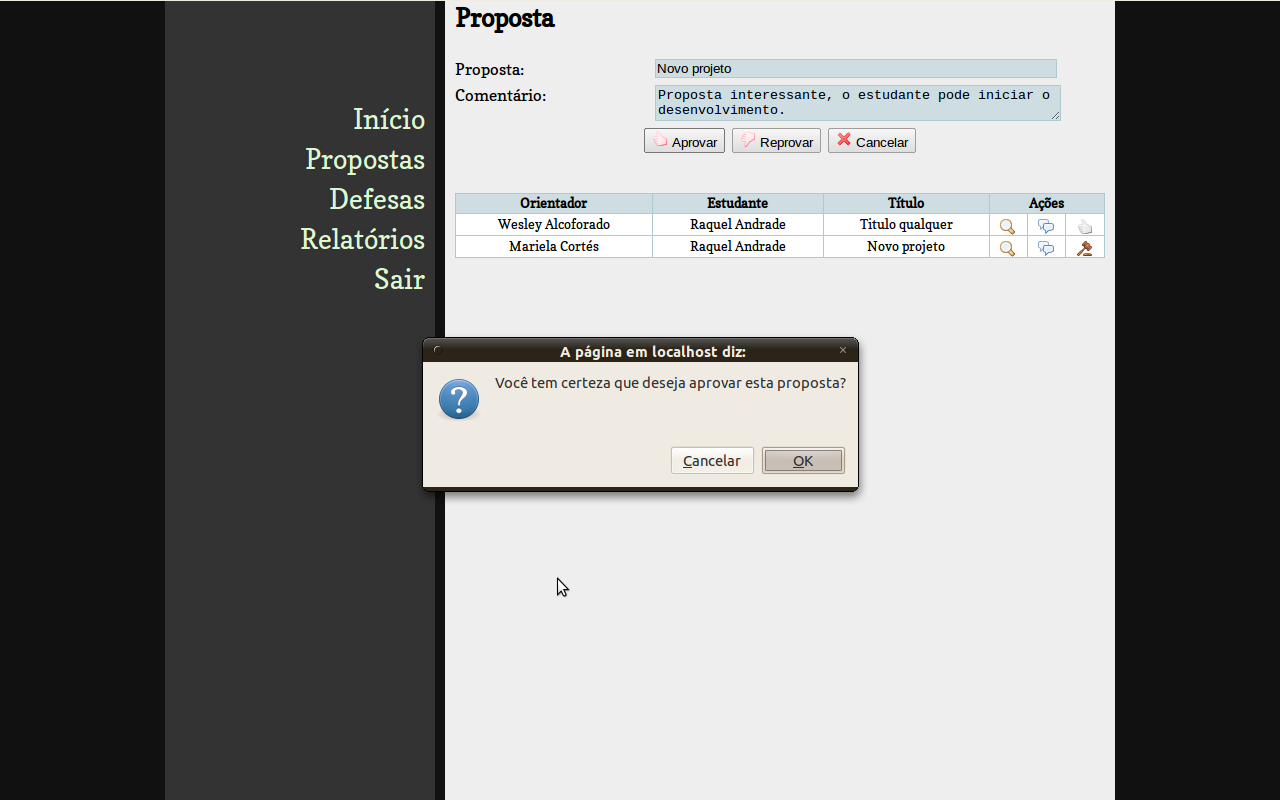
\includegraphics[width=1\textwidth]{fig/telas/processo/comissao_02_proposta_sendo_avaliada.png}
\caption{Proposta sendo avaliada pela comissão}
\label{fig:comissao_02_proposta_sendo_avaliada}
\end{figure}

\begin{figure}[htbp]
\centering
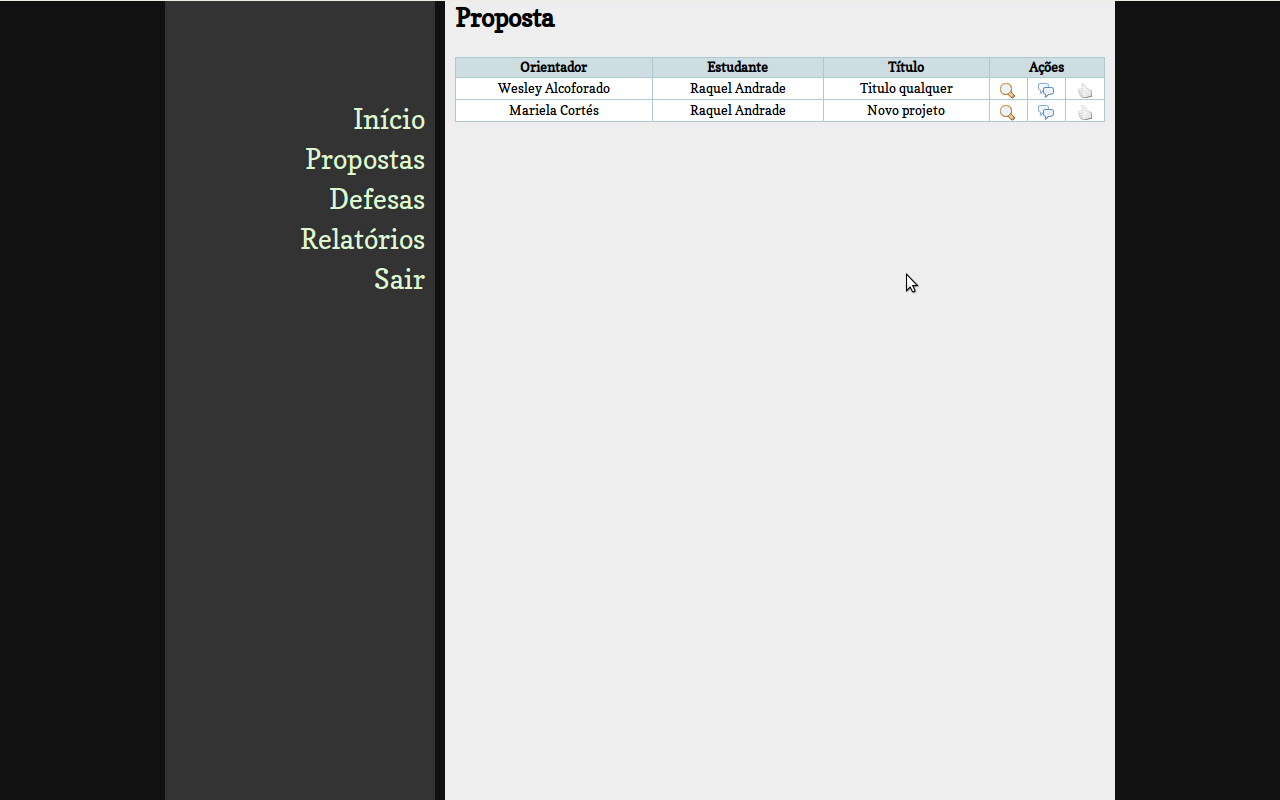
\includegraphics[width=1\textwidth]{fig/telas/processo/comissao_03_proposta_avaliada.png}
\caption{Tela de listagem de propostas após a comissão ter avaliado positivamente uma proposta}
\label{fig:comissao_03_proposta_avaliada}
\end{figure}

\begin{figure}[htbp]
\centering
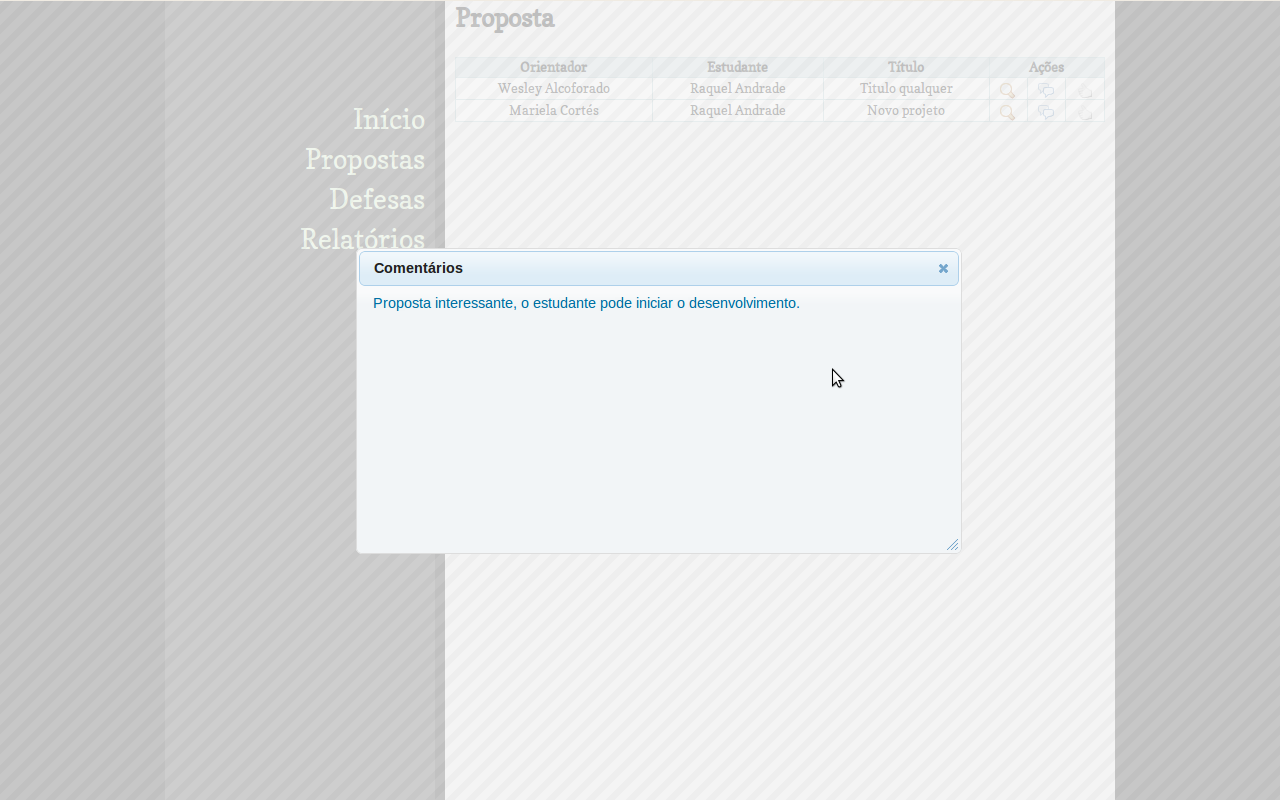
\includegraphics[width=1\textwidth]{fig/telas/processo/comissao_04_comentarios.png}
\caption{Tela de listagem de requisições de defesa submetidas pelos orientandos}
\label{fig:comissao_04_comentarios}
\end{figure}

\begin{figure}[htbp]
\centering
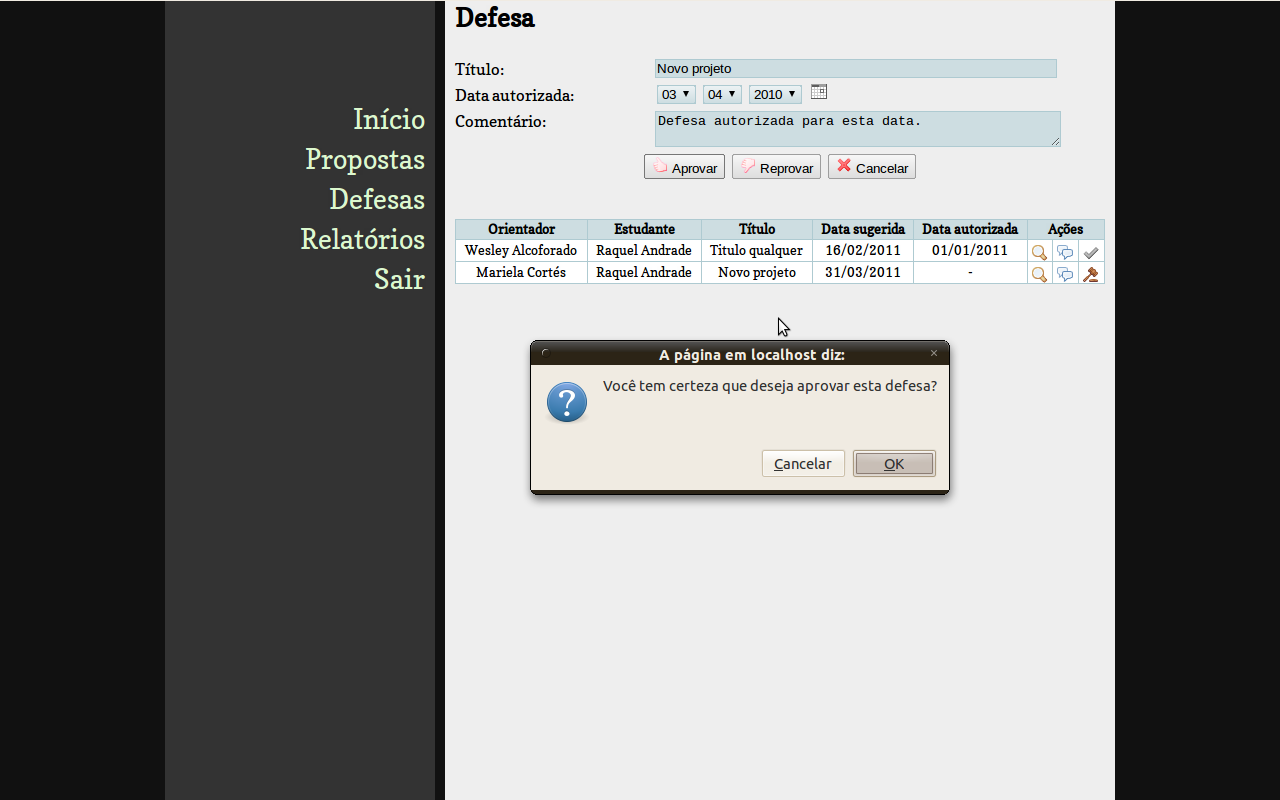
\includegraphics[width=1\textwidth]{fig/telas/processo/comissao_05_aprovando_defesa.png}
\caption{Tela de listagem de requisições de defesa no perfil da comissão}
\label{fig:comissao_05_aprovando_defesa}
\end{figure}

\begin{figure}[htbp]
\centering
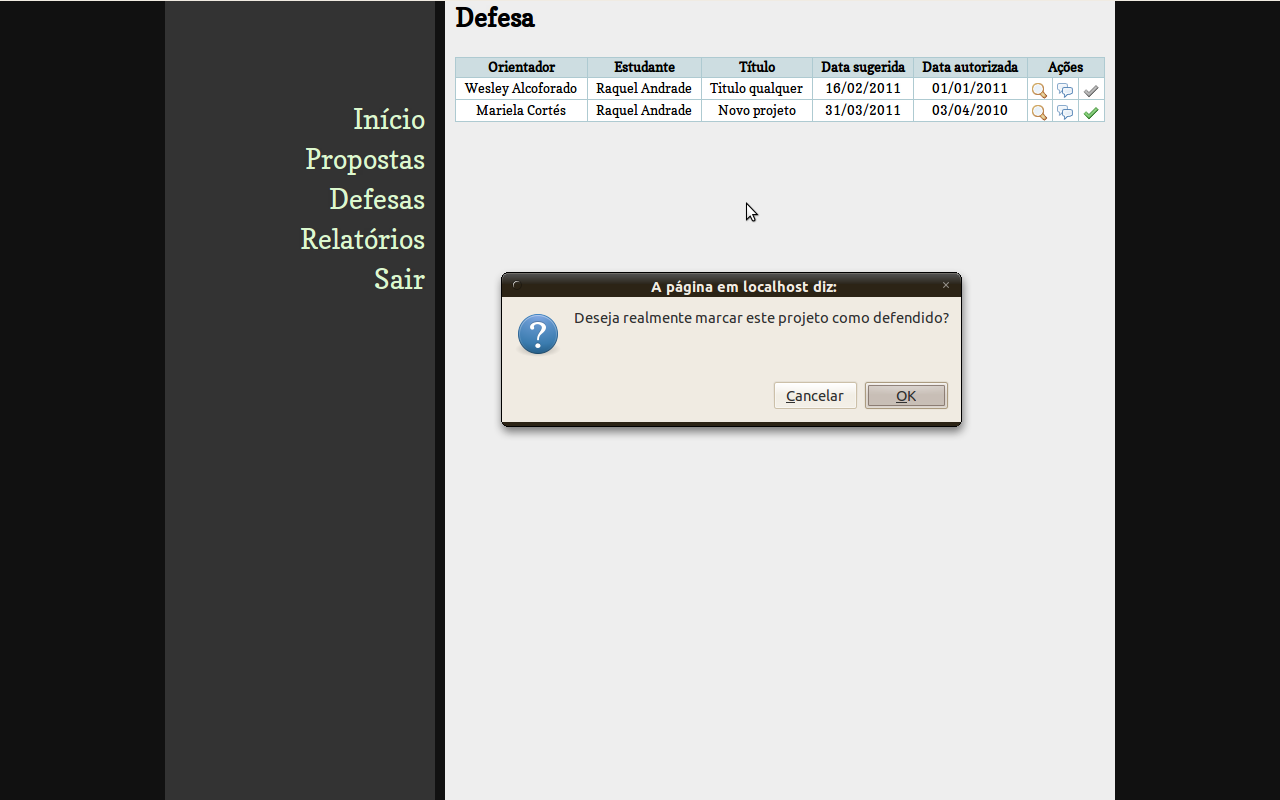
\includegraphics[width=1\textwidth]{fig/telas/processo/comissao_06_marcando_projeto_como_defendido.png}
\caption{Comissão marcando projeto como defendido}
\label{fig:comissao_06_marcando_projeto_como_defendido}
\end{figure}

